\documentclass[3p]{elsarticle}

\usepackage{lineno,hyperref}
\modulolinenumbers[5]

\journal{Journal of \LaTeX\ Templates}

%%%%%%%%%%%%%%%%%%%%%%%
%% Elsevier bibliography styles
%%%%%%%%%%%%%%%%%%%%%%%
%% To change the style, put a % in front of the second line of the current style and
%% remove the % from the second line of the style you would like to use.
%%%%%%%%%%%%%%%%%%%%%%%

%% Numbered
%\bibliographystyle{model1-num-names}

%% Numbered without titles
%\bibliographystyle{model1a-num-names}

%% Harvard
%\bibliographystyle{model2-names.bst}\biboptions{authoryear}

%% Vancouver numbered
%\usepackage{numcompress}\bibliographystyle{model3-num-names}

%% Vancouver name/year
\usepackage{numcompress}\bibliographystyle{model4-names}\biboptions{authoryear}

%% APA style
%\bibliographystyle{model5-names}\biboptions{authoryear}

%% AMA style
%\usepackage{numcompress}\bibliographystyle{model6-num-names}

%% `Elsevier LaTeX' style
\bibliographystyle{elsarticle-num}
%%%%%%%%%%%%%%%%%%%%%%%

\graphicspath{{./figure/}}




\usepackage{lineno,hyperref}

\usepackage{galois} % composition function \comp
\usepackage{bm}
\usepackage{amsmath}
\usepackage{amssymb}
\usepackage{mathrsfs}
\usepackage{amsthm}
\usepackage{natbib}
\usepackage{graphicx}
\usepackage{color}
\usepackage{booktabs}
\usepackage[page,title]{appendix}
%\renewcommand\appendixname{haha}
\usepackage{enumerate}
\usepackage{changepage}
\usepackage{datetime}
\newdate{date}{9}{1}{2017}

%%%%%%%%%% page setup %%%%%%%%%%
\textheight 8.5 in
\textwidth 6.5 in
\topmargin -0.5 in
\oddsidemargin -0.1 in
%%%%%%%%%%%%%%  Notations %%%%%%%%%%
\DeclareMathOperator{\mytr}{tr}
\DeclareMathOperator{\mydiag}{diag}
\DeclareMathOperator{\myrank}{Rank}
\DeclareMathOperator{\myP}{P}
\DeclareMathOperator{\myE}{E}
\DeclareMathOperator{\myVar}{Var}
\DeclareMathOperator*{\argmax}{arg\,max}
\DeclareMathOperator*{\argmin}{arg\,min}


\newcommand{\Ba}{\mathbf{a}}    \newcommand{\Bb}{\mathbf{b}}    \newcommand{\Bc}{\mathbf{c}}    \newcommand{\Bd}{\mathbf{d}}    \newcommand{\Be}{\mathbf{e}}    \newcommand{\Bf}{\mathbf{f}}    \newcommand{\Bg}{\mathbf{g}}    \newcommand{\Bh}{\mathbf{h}}    \newcommand{\Bi}{\mathbf{i}}    \newcommand{\Bj}{\mathbf{j}}    \newcommand{\Bk}{\mathbf{k}}    \newcommand{\Bl}{\mathbf{l}}
\newcommand{\Bm}{\mathbf{m}}    \newcommand{\Bn}{\mathbf{n}}    \newcommand{\Bo}{\mathbf{o}}    \newcommand{\Bp}{\mathbf{p}}    \newcommand{\Bq}{\mathbf{q}}    \newcommand{\Br}{\mathbf{r}}    \newcommand{\Bs}{\mathbf{s}}    \newcommand{\Bt}{\mathbf{t}}    \newcommand{\Bu}{\mathbf{u}}    \newcommand{\Bv}{\mathbf{v}}    \newcommand{\Bw}{\mathbf{w}}    \newcommand{\Bx}{\mathbf{x}}
\newcommand{\By}{\mathbf{y}}    \newcommand{\Bz}{\mathbf{z}}    
\newcommand{\BA}{\mathbf{A}}    \newcommand{\BB}{\mathbf{B}}    \newcommand{\BC}{\mathbf{C}}    \newcommand{\BD}{\mathbf{D}}    \newcommand{\BE}{\mathbf{E}}    \newcommand{\BF}{\mathbf{F}}    \newcommand{\BG}{\mathbf{G}}    \newcommand{\BH}{\mathbf{H}}    \newcommand{\BI}{\mathbf{I}}    \newcommand{\BJ}{\mathbf{J}}    \newcommand{\BK}{\mathbf{K}}    \newcommand{\BL}{\mathbf{L}}
\newcommand{\BM}{\mathbf{M}}    \newcommand{\BN}{\mathbf{N}}    \newcommand{\BO}{\mathbf{O}}    \newcommand{\BP}{\mathbf{P}}    \newcommand{\BQ}{\mathbf{Q}}    \newcommand{\BR}{\mathbf{R}}    \newcommand{\BS}{\mathbf{S}}    \newcommand{\BT}{\mathbf{T}}    \newcommand{\BU}{\mathbf{U}}    \newcommand{\BV}{\mathbf{V}}    \newcommand{\BW}{\mathbf{W}}    \newcommand{\BX}{\mathbf{X}}
\newcommand{\BY}{\mathbf{Y}}    \newcommand{\BZ}{\mathbf{Z}}    

\newcommand{\bfsym}[1]{\ensuremath{\boldsymbol{#1}}}

\def\balpha{\bfsym \alpha}
\def\bbeta{\bfsym \beta}
\def\bgamma{\bfsym \gamma}             \def\bGamma{\bfsym \Gamma}
\def\bdelta{\bfsym {\delta}}           \def\bDelta {\bfsym {\Delta}}
\def\bfeta{\bfsym {\eta}}              \def\bfEta {\bfsym {\Eta}}
\def\bmu{\bfsym {\mu}}                 \def\bMu {\bfsym {\Mu}}
\def\bnu{\bfsym {\nu}}
\def\btheta{\bfsym {\theta}}           \def\bTheta {\bfsym {\Theta}}
\def\beps{\bfsym \varepsilon}          \def\bepsilon{\bfsym \varepsilon}
\def\bsigma{\bfsym \sigma}             \def\bSigma{\bfsym \Sigma}
\def\blambda {\bfsym {\lambda}}        \def\bLambda {\bfsym {\Lambda}}
\def\bomega {\bfsym {\omega}}          \def\bOmega {\bfsym {\Omega}}
\def\brho   {\bfsym {\rho}}
\def\btau{\bfsym {\tau}}
\def\bxi{\bfsym {\xi}}
\def\bzeta{\bfsym {\zeta}}
% May add more in future.
%%%%%%%%%%%%%%%%%%%%%%%%%%%%%%%%%%%%



\theoremstyle{plain}
\newtheorem{theorem}{\quad\quad Theorem}
\newtheorem{proposition}{\quad\quad Proposition}
\newtheorem{corollary}{\quad\quad Corollary}
\newtheorem{lemma}{\quad\quad Lemma}
\newtheorem{example}{Example}
\newtheorem{assumption}{\quad\quad Assumption}
\newtheorem{condition}{\quad\quad Condition}

\theoremstyle{definition}
\newtheorem{remark}{\quad\quad Remark}
\theoremstyle{remark}

\begin{document}

\begin{frontmatter}

\title{Integrated likelihood ratio test\tnoteref{mytitlenote}}
\tnotetext[mytitlenote]{Fully documented templates are available in the elsarticle package on \href{http://www.ctan.org/tex-archive/macros/latex/contrib/elsarticle}{CTAN}.}

%% Group authors per affiliation:
\author{author \fnref{myfootnote}}
\address{Radarweg 29, Amsterdam}
\fntext[myfootnote]{Since 1880.}

%% or include affiliations in footnotes:
\author[mymainaddress,mysecondaryaddress]{Elsevier Inc}
\ead[url]{www.elsevier.com}

\author[mysecondaryaddress]{Global Customer Service\corref{mycorrespondingauthor}}
\cortext[mycorrespondingauthor]{Corresponding author}
\ead{support@elsevier.com}

\address[mymainaddress]{1600 John F Kennedy Boulevard, Philadelphia}
\address[mysecondaryaddress]{360 Park Avenue South, New York}

\begin{abstract}

    Likelihood ratio test (LRT) is the most widely used test procedure. However, it has some weaknesses. Likelihood is unbounded for some important models. Even when the likelihood is bounded, the maximum may be not easy to obtain if it is not convex in parameters. We propose a new test procedure called integrated likelihood ratio test (ILRT) which can overcome the above difficulties. Posterior Bayes factor is a special case of ILRT\@. We proof the Wilks phenomenon of ILRT and give the asymptotic local power.
\end{abstract}

\begin{keyword}
%\texttt{elsarticle.cls} \sep \LaTeX \sep Elsevier \sep template
%\MSC[2010] 00-01\sep  99-00
\end{keyword}

\end{frontmatter}

%\linenumbers

\section{Introduction}

%Suppose we are interested in  testing the hypotheses $H_0:\theta\in \Theta_0$ vs $H_1:\theta\in \Theta$ for a subset $\Theta_0$ of $\Theta$.


% Where \cite{gelfand1993bayesian} derived the null distribution of PBF.
% However, they didn't explicitly give the conditions needed. In fact, their proof relies on Laplace approximation, which assumes the existence of maximum likelihood estimator (MLE). 
% Note that the existence of MLE implies the existence of LRT. Hence the scope of their method doesn't exceed that of classical LRT\@.

%\cite{Fractional1995} proposed the fractional Bayes factor (FBF).
%The idea of fractional likelihood is also adopted by~\cite{kar10563}.
%We will see that FBF has a wider applicable scope than PBF.

%Both PBF and FBF is a special case of the general ILRT.


%Based on the proof of Bernstein-von Mises theorem (See~\cite{van2000asymptotic} and~\cite{Kleijn2012The}), we give the proof of the Wilks phenomenon and local power of ILRT under fairly weak assumptions.


%Bayesian hypothesis testing is very different from point estimation in that the data can not yanmo prior.

Suppose that we have $n$ observations $X_1,\ldots,X_n$ which are independent identically distributed (i.i.d.) random variables with values in some space space $(\mathcal{X};\mathscr{A})$.
Suppose that there is a $\sigma$-finite measure $\mu$ on $\mathcal{X}$ and that the  possible distribution $P_\theta$ of $X_i$ has a density $p(X|\theta)$ with respect to $\mu$.
Denote by $P_{\theta}^{n}$ the joint distribution of $\BX^{(n)}=(X_1,\ldots, X_n)$.
Let $p_{n}(\BX^{(n)}|\theta)=\prod_{i=1}^n p(X_i|\theta)$ denote the density of $P_{\theta}^n$ with respect to the $n$-fold product measure $\mu^n$.
The parameter $\theta$ takes its values in $\Theta$, a subset of $\mathbb{R}^{p}$.
Suppose $\theta=(\nu^T,\xi^T)^T$, where $\nu$ is a $p_0$ dimensional subvector, and $\xi$ is a $p-p_0$ dimensional subvector.
The null space $\Theta_0$ is a $p_0$-dimensional subspace of $\Theta$ defined as
\begin{equation*}
    \Theta_0=\{(\nu^T,\xi^T)^T:(\nu^T,\xi^T)^T\in\Theta, \, \xi=\xi_0\}.
\end{equation*}
 We would like to test the nested hypotheses
\begin{equation*}
    H_0:\theta\in\Theta_0\quad \text{v.s.}\quad \theta\in\Theta.
\end{equation*}
If the null hypothesis is true, we denote by $\theta_0=(\nu_0^T,\xi_0^T)^T$ the true parameter which generates the data.

The well known likelihood ratio test (LRT) is defined as
\begin{equation}
    \frac{\sup_{\Theta} p_n(\BX^{(n)}|{\theta})}{\sup_{\Theta_0} p_n(\BX^{(n)}|\theta)},
\end{equation}
where $p_n(\BX^{(n)}|\theta)=\prod_{i=1}^n p(X_i|\theta)$ is the density of $\BX^{(n)}$ with respect to $\mu^n$, the $n$-fold product measure of $\mu$.
LRT is the most widely used statistical method which enjoys many optimal properties. For example, by Neyman-Pearson lemma, it's the most powerful test (MPT) in simple null and simple alternative case \citep{Lehmann}.
In multi-dimensional parameter case, MPT does not exist.
Nevertheless, the LRT is asymptotic optimal in the sense of Bahadur efficiency \citep{MR0315820}.
However, even in some widely used models, likelihood may be unbounded. See~\cite{Cam1990Maximum} for some examples.
In this case, LRT does not exist. Another weakness of LRT occurs when the likelihood is not convex in parameters. In this case, numerical algorithms for maximizing likelihood may trap in local maxima. 



In Bayesian framework, Bayes factor is the most popular methodology.
Bayesians put prior $\pi(\nu)$ and $\pi(\theta)$ on parameters under the null and alternative hypotheses, respectively.
The conventional Bayes testing method is Bayes factor, defined as
\begin{equation*}
  \frac{\int_{\Theta} p_n(\BX^{(n)}|\theta)\pi(\theta)\, d\theta}
    {\int_{\tilde{\Theta}_0}p_n(\BX^{(n)}|\nu,\xi_0)\pi(\nu)\, d\nu},
\end{equation*}
where $\tilde{\Theta}_0=\{\nu: (\nu^T,\xi^T)^T\in \Theta_0\}$.
However, Bayes factor is sensitive to the specification of prior, which may cause difficulties in the absense of a well-formulated subjective prior. See, for example, \cite{Lindley1982}.
%The frequency property of Bayes factor is not satisfactory.
%To overcome this weakness, several robust alternatives to Bayes factor have been proposed.
To deal with this problem, several modifications of Bayes factor have been proposed.
~\cite{Aitkin1991Posterior} proposed posterior Bayes factor (PBF) which is defined to be
\begin{equation*}
    \frac{\int_{\Theta} p_n(\BX^{(n)}|\theta)\pi(\theta|\BX^{(n)})\, d\theta}{\int_{\tilde{\Theta}_0}p_n(\BX^{(n)}|\nu,\xi_0)\pi(\nu|\BX^{(n)})\, d\nu},
\end{equation*}
where $\pi(\nu|\BX^{(n)})$ and $\pi(\theta|\BX^{(n)})$ are the posterior densities under the null and alternative hypothesis, respectively.
\cite{Fractional1995} proposed fractional Bayes factor (FBF) which is defiend to be
\begin{equation*}
    \frac{L_{1}}{L_{b}}\cdot \frac{L_{b}^*}{L_{1}^*}\quad \text{for}\quad 0<b<1,
\end{equation*}
where for $t>0$,
 $$
 L_t=\int_{\Theta}\big[p_n(\BX^{(n)}|\theta)\big]^t \pi(\theta)\, d\theta,\quad
 L_t^*=\int_{\Theta_0}\big[p_n(\BX^{(n)}|\nu,\xi_0)\big]^t \pi(\nu)\, d\nu.
 $$

 The PBF and FBF can be generalized to the integrated likelihood ratio test (ILRT) statistic, as follow  
\begin{equation}
    \frac{\int_{\Theta} \big[p_n(\BX^{(n)}|\theta)\big]^{a-b}\pi(\theta;\BX^{(n)})\,d\theta}{\int_{\tilde{\Theta}_0} \big[p_n(\BX^{(n)}|\nu,\xi_0)\big]^{a-b}\pi(\nu;\BX^{(n)})\,d\nu},
\end{equation}
where $0<b<a$ are  hyperparameters,
 $\pi(\theta;\BX^{(n)})$ and $\pi(\nu;\BX^{(n)})$ be the weight functions in $\Theta$ and $\tilde{\Theta}_0$.
$\pi(\theta;\BX^{(n)})$ and $\pi(\nu;\BX^{(n)})$ may be data dependent but does not need to be the posterior density of $\theta$.
If
$$
\pi(\theta;\BX^{(n)})=\frac{\big[p_n(\BX^{(n)}|\theta)\big]^b \pi(\theta)}{\int_{\Theta}\big[p_n(\BX^{(n)}|\theta)\big]^b \pi(\theta)\, d\theta},
$$
then the ILRT equals 
$$
    \Lambda_{a,b}(\BX^{(n)})=
    \frac{L_{a}}{L_{b}}\cdot \frac{L_{b}^*}{L_{a}^*}\quad \text{for}\quad 0<b<a.
$$
We shall call $\Lambda_{a,b}(\BX^{(n)})$ the generalized FPF throughout the paper.
The FPF and PBF are both the special cases of the generalized FPF.
In fact, the FBF is equal to $\Lambda_{1,b}(\BX^{(n)})$, the PBF is equal to $\Lambda_{2,1}(\BX^{(n)})$.
Hence the ILRT is very flexible.

The paper is organized as follow.
In Section 2, we investegate the asymptotic properties of the generalzied FPF.
Section 3 consider the ILRT with general weight function.
Section 4 concludes the paper.
All technical proves are in Apppendix.


\section{Generalized FPF}
In this section, we study the asymptotic behavior of the generalized FPF.

Let $\Delta_{n,\theta_0}=\frac{1}{\sqrt{n}}\sum_{i=1}^n I_{\theta_0}^{-1}\dot{\ell}_{\theta_0}(X_i)$ be the `locally sufficient' statistics.
The corresponding quantities in the null space are 
$$\dot{\ell}^*(X)=\frac{\partial}{\partial \nu}\log p(X|\nu,\xi_0)\Big|_{\nu=\nu_0}, \quad I^*_{\theta_0}=P_{\theta_0}\dot{\ell}_{\theta_0}^*\dot{\ell}_{\theta_0}^{*T},\quad \Delta_{n,\theta_0}^*
=\frac{1}{\sqrt{n}}\sum_{i=1}^n I_{\theta_0}^{*-1}\dot{\ell}^{*}_{\theta_0}(X_i).
$$



The following assumption is adapted from~\cite{Kleijn2012The}.
\begin{assumption}\label{Assumption1}
The parameter space $\Theta$ is an open subset of $\mathbb{R}^p$. 
    The null space $\tilde{\Theta}_0$ is an open subset of $\mathbb{R}^{p_0}$.
    The parameter $\theta_0$ is an inner point of $\Theta$, $\nu_0$ is an inner point of $\tilde{\Theta}_0$.
    The function $\theta \mapsto \log p(X|\theta)$ is differentiable at $\theta_0$  $P_{\theta_0}$-a.s.\ with derivative 
$$\dot{\ell}_{\theta_0}(X)=\frac{\partial}{\partial \theta}\log p(X|\theta)\Big|_{\theta=\theta_0}.$$
There's an open neighborhood $V$ of $\theta_0$ such that for every $\theta_1,\theta_2\in V$,
        \begin{equation*}
            |\log p(X|\theta_1)-\log p(X|\theta_2)|\leq m(X)\|\theta_1-\theta_2\|,
        \end{equation*}
        where $m(X)$ is a measurable function satisfying $P_{0}\exp[s m(X)]<\infty$ for some $s>0$.
        The Fisher information matrix $I_{\theta_0}=P_{\theta_0}\dot{\ell}_{\theta_0}\dot{\ell}_{\theta_0}^T$ is positive-definite and as $\theta\to \theta_0$,
    \begin{equation*}
        P_{\theta_0} \log \frac{p(X|\theta)}{ \log (X|\theta_0)}
        =-\frac{1}{2}(\theta-\theta_0)^T I_{\theta_0} (\theta-\theta_0)+o(\|\theta-\theta_0\|^2).
    \end{equation*}
\end{assumption}     
Assumption~\ref{Assumption1} is satisfied by many common models, it ensures a local asymptotic normality expansion of likelihood. See Lemma~\ref{Thm:localExpansion} in Appendix.

    For $t>0$, we say $L_t$ is $\sqrt{n}$-consistent if for every $M_n\to \infty$,
    $$
    \frac{L_t({\{\theta:\|\theta-\theta_0\|> M_n/\sqrt{n}\}})}{L_t}\xrightarrow{P_{\theta_0}^n} 0,
    $$
    where for a set $A\subset \Theta$,
$$
L_t (A)=\int_{A} \Big[ {p_n(\BX^{(n)}|\theta)} \Big]^{t} \pi(\theta) \, d \theta.
$$
The $\sqrt{n}$-consistency of $L_t^*$ is defined similarly.
    Note that the consistency of $L_1$ is equivalent to the consistency of the posterior distribution.
    In~\cite{Kleijn2012The}, the $\sqrt{n}$-consistency of posterior distribution is a key assumption to prove Bernstein-von Mises theorem.
    Likewise, the $\sqrt{n}$-consistency of $L_t$ is a key assumption of the following theorem.



    \begin{theorem}\label{Thm:maintheorem}
        Suppose that Assumption~\ref{Assumption1} holds, $L_a$, $L_b$, $L_a^*$ and $L_b^*$ are $\sqrt{n}$-consistent, $\pi(\theta)$ is continuous at $\theta_0$ with $\pi(\theta_0)>0$, $\pi(\nu)$ is continuous at $\nu_0$ with $\pi(\nu_0)>0$, then
        for $\{\theta_n\}$ such that $\sqrt{n}(\theta_n-\theta_0)\to \eta$, 
        $$
        2\log \Lambda_{a,b}(\BX^{(n)})\overset{P^n_{\theta_n}}{\rightsquigarrow}-{(p-p_0)}\log \frac{a}{b}+{(a-b)}\chi^2_{p-p_0}(\delta),
        $$
        where $\chi^2_{p-p_0}(\delta)$ is a noncentral chi-squared random variable with $p-p_0$ degrees of freedom and noncentrality parameter $\delta=\eta^T\big( I_{\theta_0}-I_{\theta_0} J(J^T I_{\theta_0} J)^{-1}J^T I_{\theta_0}\big)\eta$ and $J=(I_{p_0},0_{p_0\times(p-p_0)})^T$,
``$\rightsquigarrow$'' means weak convergence.
    \end{theorem}
Theorem~\ref{Thm:maintheorem} gives the asymptotic distribution of $2\log \Lambda_{a,b}(\BX^{(n)})$ under the null hypothesis and the local alternative hypothesis.
To obtain a test with asymptotic level $\alpha$, the critical value of $2\log \Lambda_{a,b}(\BX^{(n)})$ can be defined to be $-(p-p_0)\log (a/b)+ (a-b)\chi^2_{p-p_0,1-\alpha}$, where $\chi^2_{p-p_0,1-\alpha}$ is the $1-\alpha$ quantile of a chi-squared random variable with $p-p_0$ degrees of freedom.
The resulting test has local asymptotic power
\begin{equation}\label{eq:likelihoodPower}
\Pr \big( \chi^2_{p-p_0}(\delta)> \chi^2_{p-p_0,1-\alpha} \big).
\end{equation}
It is known that, under certain regular conditions,~\eqref{eq:likelihoodPower} is also the local asymptotic power of the likelihood ratio test. 
In this view, $\Lambda_{a,b}(\BX^{(n)})$ enjoys good frequentist properties.


 The $\sqrt{n}$-consistency of $L_t$ plays a key role in the proof of \ref{Thm:maintheorem}.
We would like to give sufficient conditions for the $\sqrt{n}$-consistency of $L_t$.
 The following proposition shows that for full-rank exponential family, $L_t$ is $\sqrt{n}$-consistent for all $t>0$.
\begin{proposition}\label{exponentialCon}
    Suppose $p(X|\theta)=\exp\big[\theta^T T(X)-A(\theta)\big]$, $\Theta$ is an open subset of $\mathbb{R}^p$, $\theta_0$ is an interior point of $\Theta$, 
    $$I_{\theta_0}=\frac{\partial^2}{\partial \theta \partial \theta^T} A(\theta_0)>0.$$
    Then $L_{t}$ is consistent for $t>0$.
\end{proposition}


 In general case, however, the $\sqrt{n}$-consistency of $L_t$ needs further conditions.
 For $t=1$, the $\sqrt{n}$-consistency of $L_t$ is equivalent to the $\sqrt{n}$-consistency of posterior distribution.
 The consistency of posterior distribution have been considerable attention in the literature.
 See, for example,~\cite{ghosal2000},~\cite{Shen2001Rates},~\cite{vaart2007convergence} and the references therein.
A popular and convenient way of establishing the consistency of posterior is through the condition that suitable test sequences exist.
This approach is adopted by~\cite{ghosal2000},~\cite{vaart2007convergence} and~\cite{Kleijn2012The}.

\begin{assumption}\label{Assumption2}
    For every $\epsilon>0$, there exists a sequence of tests $\phi_n$ such that
        \begin{equation}
            P_{\theta_0}^n\phi_n\to 0,\quad \sup_{\|\theta-\theta_0\|\geq \epsilon} P_\theta^n(1-\phi_n)\to 0.
        \end{equation}
\end{assumption}

\begin{proposition}[\cite{Kleijn2012The}, Theorem 3.1]
    Suppose $\theta_0$ is an interior of $\Theta$, $\pi(\theta)$ is continuous at $\theta_0$ and $\pi(\theta_0)>0$.
    Under Assumptions \ref{Assumption1} and~\ref{Assumption2}, $L_1$ is consistent.
\end{proposition}
Assumption~\ref{Assumption2} is satisfied when the parameter space is compact and the model is suitably continuous. See Theorem 3.2 of~\cite{Kleijn2012The}.

The consistency of $L_t$ for $0<t<1$ is different from the consistency of posterior distribution.
\cite{kar10563} considered the Hellinger consistency of $L_{1/2}$.
However, they only consider $t=1/2$ and didn't prove the $\sqrt{n}$-convergence result.
Next we shall prove the consisency of $L_{t}$ for $0<t<1$ under certain conditions on the R\'{e}nyi divergence between distributions in the family $\{P_\theta:\theta\in\Theta\}$.

 For two parameters $\theta_1$ and $\theta_2$, the $\alpha$ order R\'{e}nyi divergence ($0<\alpha<1$) of $P_{\theta_1}$ from $P_{\theta_2}$ is defined to be
$$
D_{\alpha}(\theta_1||\theta_2)=-\frac{1}{1-\alpha}\log \rho_{\alpha}(\theta_1,\theta_2),
$$
where
$
\rho_{\alpha}(\theta_1,\theta_2)=\int_{\mathcal{X}} p(X|\theta_1)^{\alpha} p(X|\theta_2)^{1-\alpha} \, d \mu
$ is the so-called Hellinger integral.
The following assumption will be assumed in our $\sqrt{n}$-consistency result.
\begin{assumption}\label{Assumption4}
    For some $\alpha\in(0,1)$, there exist positive constancts $\delta$, $\epsilon$ and $C$ such that,
     $D_{\alpha}(\theta||\theta_0)  \geq  C \|\theta-\theta_0\|^2$ for $\|\theta-\theta_0\|\leq \delta$ and $D_{\alpha}(\theta||\theta_0) \geq \epsilon$ for $\|\theta-\theta_0\|>\delta$.
\end{assumption}
\begin{remark}
    A remarkable property of R\'{e}nyi divergence is the equivalence of all $D_{\alpha}$: If $0<\alpha<\beta<1$, then
    $$
    \frac{\alpha}{1-\alpha}\frac{1-\beta}{1-\alpha} D_{\beta}(\theta_1||\theta_2)
    \leq D_{\alpha}(\theta_1||\theta_2)\leq D_{\beta}(\theta_1||\theta_2).
    $$
    See, for example,~\cite{2016arXiv160801805B}.
    As a result, if Assumption~\ref{Assumption4} holds for some $\alpha\in(0,1)$, then it will hold for every $\alpha\in(0,1)$.
\end{remark}
To appreciate Assumption~\ref{Assumption4},
   suppose, for example, that $D_{\alpha}(\theta||\theta_0)$ is twice continuously differentiable in $\theta$.
   Since $\theta=\theta_0$ is a minumum point of  $D_{\alpha}(\theta||\theta_0)$, the first order derivative of $D_{\alpha}(\theta||\theta)$ at $\theta=\theta_0$ is zero and the second order derivative at $\theta=\theta_0$ is positive semidefinite.
By Taylor theorem, in a small neighbourhood of $\theta_0$,
   $$
   D_{\alpha}(\theta||\theta_0)=\frac{1}{2}(\theta-\theta_0)^T \frac{\partial^2}{\partial \theta \partial \theta^T} D_{\alpha}(\theta||\theta_0)\Big|_{\theta=\theta^*}  (\theta-\theta_0),
   $$
   where $\theta^*$ is between $\theta_0$ and $\theta$.
   If we further assume the second order derivative is positive definite at $\theta=\theta_0$, then in a small neighbourhood of $\theta_0$, there is a positive constant $C$ such that $D_{\alpha(\theta||\theta_0)}\geq C\|\theta-\theta_0\|^2$.
   Thus, Assumption~\ref{Assumption4} is a fairly weak condition.
\begin{proposition}\label{Theoremless1}
    Suppose $\theta_0$ is an interior of $\Theta$, $\pi(\theta)$ is continuous at $\theta_0$ and $\pi(\theta_0)>0$.
    Under Assumptions \ref{Assumption1} and~\ref{Assumption4}, for fixed $t\in(0,1)$, $L_t$ is consistent.
\end{proposition}
The consistency of $L_t$ for $t>1$ can be proved under conditions similar to Assumption~\ref{Assumption2}.
However, while we require $\{\phi_n\}$ to be consistent tests, the requirement on the sequence $\{\phi_n\}$ for $t>1$ lacks statistical interpretation.
This implies that it may not be natural to use $L_t$ for $t>1$.

Note that $L_1$ is always well defined since it has finite integral.
By holder inequality, $L_{t}$ is also well defined for $0<t<1$.
However, $L_t$ is not always well defined.
The following example is a counterexample.

\begin{example}
Suppose $X_1,\ldots,X_n$ are i.i.d. from the density
$$
    p(x|\theta)=C |x-\theta|^{-1/2}\exp\big[-(x-\theta)^2\big]
,
$$
    where $C$ is the normalizing constant. The parameter space $\Theta$ is equal to $\mathbb{R}$.
    We would like to test the hypotheses $H_0:\theta=0$ vs $H_1:\theta\neq 0$.
    The likelihood is
    $$
    p_n(\BX^{(n)}|\theta)=C^n \Big[\prod_{i=1}^n |X_i-\theta|\Big]^{-1/2}
    \exp \big[-\sum_{i=1}^n (X_i-\theta)^2 \big].
    $$
    Under the alternative hypothesis, the likelihood tends to infinity if $\theta$ tends to $X_i$, $i=1,\ldots, n$.
    Consequently, LRT fails in this model.
    We impose a prior $\pi(\theta)$.
    Suppose that $\pi(\theta)$ is positive for all $\theta$.
Then
$$
    \begin{aligned}
        L_t(\BX^{(n)})=&
    \int_{-\infty}^{+\infty}
\Big[\prod_{i=1}^n |X_i-\theta|\Big]^{-t/2}
    \exp \big[-t\sum_{i=1}^n (X_i-\theta)^2 \big]
        \pi(\theta)
    \,
    d \theta.
    \end{aligned}
$$
    The likelihood will almost surely have no ties and consequently $L_t(\BX^{(n)})=+\infty$ if and only if $t\geq 2$.
\end{example}



\section{General weight function}


In some cases, the posterior density or the general FBF is not easy to calculate or have unsatisfactory properties.
Thanks to the flexibility of ILRT, we can consider general weight function in such cases.

Let $h=\sqrt{n}(\theta-\theta_0)$. \cite{Kleijn2012The}, Theorem 2.1 states that
under Assumption~\ref{Assumption1},~\ref{Assumption2},
$$
            \|\pi_n(h|\BX^{(n)})-\phi(h;\Delta_{n,\theta_0},I_{\theta_0}^{-1})\|\overset{P_{\theta_0}^n}{\to}0,
$$
where for two density $p$ and $q$, $\|p-q\|=\int |p-q|$ is the total variation distance between $p$ and $q$.
We shall assume that the weight function inherits this property.
        
\begin{assumption}\label{Assumption3}
    Let $\pi_n(h;\BX^{(n)})$ be a weight function satisfying 
        \begin{equation}\label{vonMisesResults}
            \|\pi_n(h;\BX^{(n)})-\phi(h;\Delta_{n,\theta_0},I_{\theta_0}^{-1})\|\overset{P_{\theta_0}^n}{\to}0
        \end{equation}
Furthermore, assume that for every $\epsilon>0$, there's a Lebesgue integrable function $T(h)$, a $K>0$ and an $A>0$ such that 

    \begin{equation}\label{Assump31}
        \lim_{n\to \infty}P_{\theta_0}^n(\sup_{\|h\|\geq K\sqrt{n}}(\pi_n(h;\BX^{(n)})-T(h))\leq 0)\geq 1-\epsilon
\end{equation}

        \begin{equation}\label{Assump32}
            \lim_{n\to \infty} P_{\theta_0}^n(\sup_{\|h\|\leq K\sqrt{n}} \pi_n(h;\BX^{(n)})\leq A)\geq 1-\epsilon
        \end{equation}
\end{assumption}


The condition~\ref{Assump31} assumes there is a function controlling the tail of weight function. For a statistical model, the likelihood value makes no sense when $\theta$ is far away from $\theta_0$, or $\sqrt{n}h$ is large.
The bad behavior of the tail of likelihood function may affect the behavior of posterior distribution.
To avoid the bad behavior of the likelihood function when $\sqrt{n}h$ is large, most existing literatures impose conditions on the model.
Here we impose~\ref{Assump31} on weight function instead.
The condition~\ref{Assump32} is satisfied in most usual case.

\begin{theorem}\label{theoremMain}
    Suppose the true parameter $\theta_0$ is an interior point of $\Theta$, $\nu$ is a relative interior point of $\tilde{\Theta}_0$.
    Under Assumptions~\ref{Assumption1},~\ref{Assumption2} and\ref{Assumption3}, for bounded real numbers $\eta_n$, we have

    $$
    2\log(\Lambda(X))\overset{P_{{\eta_n}}^n}{\rightsquigarrow} -(p_2-p_1)\log 2+\chi^2_{p_2-p_1}(\delta)
    $$
    %\begin{equation}
        %\Big|\int_{\mathbb{R}^{p}}\frac{p_n(\BX^{(n)}|\theta_0+n^{-1/2}h)}{p_n(\BX^{(n)}|\theta_0)}\pi_n(h;\BX^{(n)})\,dh-
        %2^{-\frac{p}{2}}\exp\big[\frac{1}{2}\Delta_{n,\theta_0}^T I_{\theta_0}\Delta_{n,\theta_0}\big]
        %\Big|\xrightarrow{P_{\eta_n}^n}0.
    %\end{equation}
\end{theorem}

A practical method to obtain simple form weight function $\pi_n(h;\BX^{(n)})$ is the variational inference. See, for example,~\cite{blei2017}.
The following example shows that the weight function obtained from R\'{e}nyi divergence variational inference satisfies Assumption~\ref{Assumption3}.

\begin{example}
    Suppose $\pi_n(h;\BX^{(n)})$ is obtain from R\'{e}nyi divergence variational inference~\citep{NIPS2016_6208}:
    $$
        \pi_n(h;\BX^{(n)})=\min_{q\in\mathcal{Q}} -\frac{1}{1-\alpha} \log \int_{\mathcal X} q(h)^{\alpha} \pi(h|\BX^{(n)})^{1-\alpha}\, d\mu,
    $$
    where $\mathcal{Q}$ is the family of all $p$ dimensional normal distribution.
    Since
    \begin{equation}\label{eq:xiebuwan}
    -\frac{1}{1-\alpha} \log \int_{\mathcal X} \pi(h;\BX^{(n)})^{\alpha} \pi(h|\BX^{(n)})^{1-\alpha}\, d\mu
    \leq
    -\frac{1}{1-\alpha} \log \int_{\mathcal X} \phi(h;\Delta_{n,\theta_0}, I_{\theta_0}^{-1})^{\alpha} \pi(h|\BX^{(n)})^{1-\alpha}\, d\mu.
    \end{equation}
    By the equivalence of R\'{e}nyi divergence and total variation distance and Bernstein-von Mise theorem, the right hand side of~\eqref{eq:xiebuwan} tends to $0$.
    Again by the equivalence of R\'{e}nyi divegence and total variation distance,~\eqref{vonMisesResults} holds.
    Since $\pi_n(h;\BX^{(n)})$ is a normal density,~\eqref{vonMisesResults} implies the mean and covariance parameter of $\pi_n(h;\BX^{(n)})$ converges to $\Delta_{n,\theta_0}$ and $I_{\theta_0}^{-1}$ respectively. Then~\eqref{Assump31} and~\eqref{Assump32} hold.
\end{example}


\section{Conclusion}
In this paper, we proposed a flexible methodology ILRT which includes some existing method as special cases.
We gave the asymptotic distribution of the generalized FPF, which is a special case of ILRT.
We also investigates the asymptotic behavior of ILRT for general weight functions.
This allows one to use a simple form approximation of the posterior distribution as weight function.
In particular, we show that the weight function can be obtained from R\'{e}nyi divergence variational inference.

\section*{Acknowledgements}
This work was supported by the National Natural Science Foundation of China under Grant No. 11471035, 11471030.




%Suppose  the Assumptions of~\ref{theoremWilks} are met. The true parameter $\theta$ satisfies $\eta_n=\sqrt{n}(\theta-\theta_0)\to \eta$. If
%\begin{equation}
    %I_{\theta_0}=\left(
        %\begin{matrix}
            %I^*_{\theta_0}&I_{12}
            %\\
            %I_{21}&I_{22}
        %\end{matrix}
    %\right),
%\end{equation}
%$I_{22\cdot 1}=I_{22}-I_{21}I_{\theta_0}^{*-1}I_{12}$,
    %then we have
%\begin{equation}
    %2\log(\Lambda(X))\overset{P_0^n}{\rightsquigarrow} \chi^2_{p_2-p_1}(\delta)-(p_2-p_1)\log(2)
%\end{equation}
%where
%\begin{equation}
%\delta=\eta^T
    %\left(
        %\begin{matrix}
            %0&0\\
            %0&I_{22\cdot 1}
        %\end{matrix}
    %\right)
    %\eta
%\end{equation}
%\end{theorem}
%
%The results can be explained by the limit experiment point of view. As $h_n\to h$, the `locally sufficient' statistic $\Delta_{n,\theta_0}\rightsquigarrow N(h,I^{-1}_{\theta_0})$. In the limit experiment, we have one observation $X\sim N(h,I_{\theta_0}^{-1})$. In this case, the integrated likelihood ratio test statistics can be calculated easily whose distribution is exactly the same as~\ref{theoremPower}.
%

%\begin{proof}[\textbf{Proof of Theorem~\ref{theoremPower}}]
    %We note that $h_n=\eta_n$ converges to $\eta$. By Proposition~\ref{Thm:localExpansion} and CLT,
%\begin{equation}
    %\begin{aligned}
    %\left(
    %\begin{matrix}
        %\frac{1}{\sqrt{n}}\sum^n_{i=1}\dot{\ell}_{\theta_0}(X_i)
        %\\
        %\log \frac{p_{\eta_n}(X)}{p_0(X)}
    %%\end{matrix}
    %\right)
    %&=\left(
        %\begin{matrix}
        %\frac{1}{\sqrt{n}}\sum^n_{i=1}\dot{\ell}_{\theta_0}(X_i)
        %\\
        %\frac{1}{\sqrt{n}}\sum^n_{i=1}\eta^T\dot{\ell}_{\theta_0}(X_i)-\frac{1}{2}\eta^T I_{\theta_0}\eta
        %\end{matrix}
    %\right)
    %+o_{P_0^n}(1)\\
    %&\overset{P_0^n}{\rightsquigarrow}
    %N(
    %\left(
    %\begin{matrix}
        %0\\
        %-\frac{1}{2}\eta^T I_{\theta_0}\eta
    %\end{matrix}
    %\right),
    %\left(
        %\begin{matrix}
            %I_{\theta_0}&I_{\theta_0}\eta\\
            %\eta^T I_{\theta_0}&\eta^T I_{\theta_0}\eta
        %\end{matrix}
    %\right)
    %).
    %\end{aligned}
%\end{equation}
%Hence by Le Cam's third lemma,
%\begin{equation}
    %\frac{1}{\sqrt{n}}\sum^n_{i=1}\dot{\ell}_{\theta_0}(X_i)\overset{P^n_{\eta_n}}{\rightsquigarrow}\xi\sim N(I_{\theta_0}\eta,I_{\theta_0}).
%\end{equation}
%By Theorem~\ref{theoremMain}, under $P_{\eta_n}^n$, we have~\eqref{equationNull}.
%Hence
%\begin{equation}
    %2\log(\Lambda(X))\overset{P_{\eta_n}^n}{\rightsquigarrow} \chi^2_{p_2-p_1}(\delta)-(p_2-p_1)\log(2),
%\end{equation}
%where noncentral parameter $\delta$ can be obtained by substituting $\xi$ by $I_{\theta_0}\eta$ in~\eqref{equationXi}:
%\begin{equation}
    %\begin{aligned}
        %\delta&=\eta^T(
        %I_{\theta_0}-
        %I_{\theta_0}
        %\left(\begin{matrix} 
                %I^{*-1}_{\theta_0}&0\\
                %0&0
        %\end{matrix}\right)
        %I_{\theta_0}
    %)\eta
    %\\
    %&=\eta^T
    %\left(
        %\begin{matrix}
            %0&0\\
            %0&I_{22\cdot 1}
        %\end{matrix}
    %\right)
    %\eta.
    %\end{aligned}
%\end{equation}
%\end{proof}







%
\section{Normal mixture}

 Normal mixture is the first example of unbounded likelihood given in~\cite{Cam1990Maximum}. In this section, we apply ILRT to this model.


Suppose $X_1,\ldots,X_n$ are i.i.d.\ distributed as a mixture of normal distributions
\begin{equation}
    p_\theta(x)=\frac{1-\alpha}{\sqrt{2\pi}}\exp\left\{-\frac{1}{2}{(x-\mu)}^2\right\}+
    \frac{\alpha}{\sigma\sqrt{2\pi}}\exp\left\{-\frac{1}{2}\frac{{(x-\mu)}^2}{\sigma^2}\right\},
\end{equation}
 where $\alpha$ is a known constant. Suppose the parameter space is
\begin{equation}
    \Theta=\{\theta={(\mu,\sigma^2)}^T:\mu\in(\-\infty,\infty),\sigma^2\in (0,M)\},
\end{equation}
where $M$ is a sufficiently large parameter.
\cite{Cam1990Maximum} pointed out that the likelihood of the model is unbounded. In fact, let $\mu=X_1$ and let $\sigma^2\to 0$, then the likelihood tends to infinity.

Under the model, we consider testing the hypotheses $H_0:\mu=0,\sigma=2$ vs $H_1:\theta\in
\Theta$. Although LRT fails in this model, ILRT can still be used. In fact, we can verify (although cumbersome) that $(i)$, $(ii)$ and $(iii)$ all hold. Hence Theorem~\ref{theoremWilks} and~\ref{theoremPower} hold. To use ILRT, we need a weight function.
First let the weight function be the posterior density of parameters. To make the posterior density bounded from infinity, we consider the so-called zero-avoiding prior (see~\cite{bayesianDataAnalysis} section 13.2).
When $\mu=X_1$, as $\sigma^2\to 0$, the likelihood tends to infinity at the rate of ${1}/{\sigma}$. The rate can be hedged by the density of $\chi^2(3)$. Hence we adopt the following prior distribution

\begin{equation}
    dN(0,1)(\mu)\times d\chi^2(3)(\sigma^2),
\end{equation}
where $d\chi^2(3)(\sigma^2)$ represents the density of $\chi^2$ distribution with freedom $3$ taking value at $\sigma^2$. Because the $\sigma^2$ is limited in $(0,M)$, we also truncate prior of $\sigma^2$ at $M$.

We next verify the Wilks phenomenon by simulation. We take sample size $n=50,100,200$ and $\alpha=0.1,0.5,0.9$. In every combination, we repeat $1000$ samples and obtain $1000$ ILRT statistics. We expect the empirical distribution is similar to that of $\chi^2(2)$. We plot the QQ-plot of empirical distribution relative to  $\chi^2(2)$ distribution, it can be seen that ILRT can be well approximated by $\chi^2(2)$.

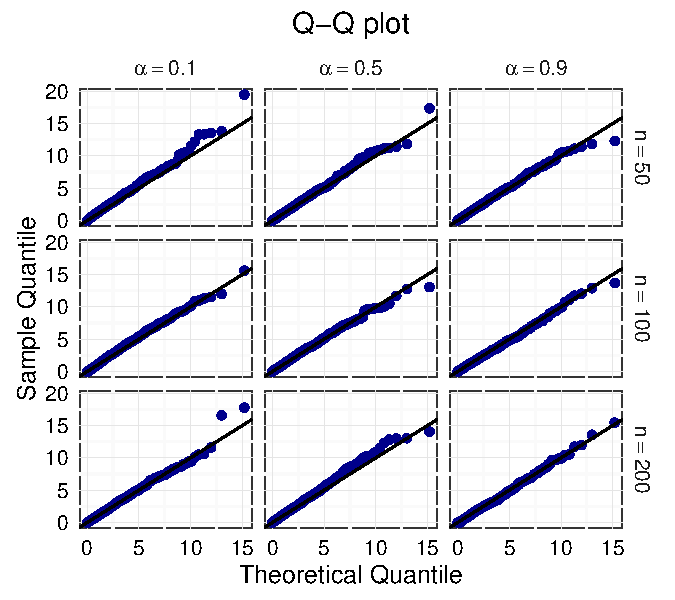
\includegraphics{myQQPlot.pdf}


We next consider another weight function $\pi (\theta; X)= N(\hat{\theta},\frac{1}{n}\hat{I}^{-1}_{\hat{\theta}})$. Lt $\hat{\theta}$ be the highest probability density estimator. And 
$$\hat{I}_\theta^{-1}=\sum_{i=1}^n
\begin{bmatrix}
-\frac{\partial^2 \log p_\theta(x_i)}{\partial \mu^2}&
    -\frac{\partial^2 \log p_\theta(x_i)}{\partial \mu\partial (\sigma^2)}
\\
    -\frac{\partial^2 \log p_\theta(x_i)}{\partial \mu\partial (\sigma^2)}
    &
    -\frac{\partial^2 \log p_\theta(x_i)}{\partial {(\sigma^2)}^2}
\end{bmatrix}$$
where

\begin{equation}
    \begin{aligned}
\frac{\partial^2 \log p_\theta(x)}{\partial
        \mu^2}=&
        \frac{(1-\alpha)({(x-\mu)}^2-1)dN(\mu,1)(x)+\alpha ({(x-\mu)}^2/\sigma^4 -\sigma^{-2})dN(\mu,\sigma^2)(x)}{p_\theta (x)}-\\
        &
        {\Big(\frac{(1-\alpha)(x-\mu)dN(\mu,1)(x)+\alpha(x-\mu)/\sigma^2 dN(\mu,\sigma^2)(x)}{p_\theta(x)}\Big)}^2,
    \end{aligned}
\end{equation}

\begin{equation}
    \begin{aligned}
        &\frac{\partial^2 \log p_\theta(x)}{\partial
        \mu\partial(\sigma^2)}=
        \frac{(\frac{3\alpha(\mu-x)}{2\sigma^4}-\frac{\alpha {(\mu-x)}^3}{2\sigma^6})dN(\mu,\sigma^2)(x)}{p_\theta (x)}-\\
        &
        \frac{\alpha (\frac{{(\mu-x)}^2}{2\sigma^4}-\frac{1}{2\sigma^2})dN(\mu,\sigma^2)(x)\big((1-\alpha)(x-\mu)dN(\mu,1)(x)+\alpha(x-\mu)/\sigma^2 d(\mu,\sigma^2)(x)\big)}{p_{\theta}{(x)}^2},
    \end{aligned}
\end{equation}


\begin{equation}
    \begin{aligned}
\frac{\partial^2 \log p_\theta(x)}{\partial
        {(\sigma^2)}^2}=&
        \frac{\alpha \big(\frac{3}{4\sigma^4}-\frac{3{(x-\mu)}^2}{2\sigma^6} +\frac{{(x-\mu)}^4}{4\sigma^8}\big)dN(\mu,\sigma^2)(x)}{p_\theta (x)}-\\
        &
        {\Big(\frac{\alpha\big(\frac{{(x-\mu)}^2}{2\sigma^4}-\frac{1}{2\sigma^2} \big)dN(\mu,\sigma^2)(x)}{p_\theta(x)}\Big)}^2.
    \end{aligned}
\end{equation}

We do the same simulation as above and the QQ-plot is given.
It  can be seen that the Wilks phenomenon still holds in this case.
For mixture model, sampling from posterior distribution is troublesome.
The computing burden will be reduce by normal approximation.
This is an advantage of normal weight ILRT.\@ From this example, we can see that ILRT is more flexible than posterior Bayes factor.


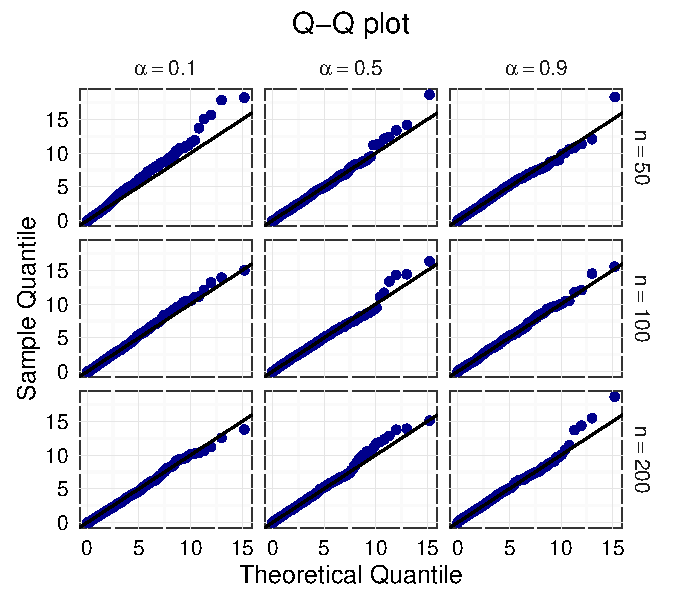
\includegraphics{myQQPlotNormal.pdf}





\begin{appendices}
For two measure sequence $P_n$ and $Q_n$ on measurable spaces $(\Omega_n,\mathcal{A}_n)$, denote by $P_n\triangleleft \triangleright Q_n$ that $P_n$ and $Q_n$ are mutually contiguous. That is, for any statistics $T_n$: $\Omega_n\mapsto \mathbb{R}^k$, we have $T_n\overset{P_n}{\rightsquigarrow}0\Leftrightarrow T_n\overset{Q_n}{\rightsquigarrow}0$.

\begin{lemma}[\cite{Kleijn2012The}, Lemma 2.1.]\label{Thm:localExpansion}
    Under Assumption~\ref{Assumption1},
    we have $\|\dot{\ell}_{\theta_0}(X)\|\leq m(X)$ $P_0$-a.s., $P_0 \dot{\ell}_{\theta_0}(X)=0$ and for every $M>0$
    \begin{equation*}
        \sup_{\|h\|\leq M}\Big|
         \log \frac{p_n(\BX^{(n)}|\theta_0+n^{-1/2}h)}{p_n(\BX^{(n)}|\theta_0)}-h^T I_{\theta_0}\Delta_{n,\theta_0}+\frac{1}{2}h^T I_{\theta_0}h
        \Big|\xrightarrow{P^n_0}0.
    \end{equation*}
    %(See~\cite{van2000asymptotic} Theorem 5.23 or)
\end{lemma}

\begin{lemma}\label{Thm:someTest}
    Under Assumptions~\ref{Assumption1} and~\ref{Assumption2},
    there exists for every $M_n\to \infty$ a sequence of tests $\phi_n$ and a constant $\delta>0$ such that, for every sufficiently large $n$ and every $\|\theta-\theta_0\|\geq M_n/\sqrt{n}$,
    $$
    P^n_{0} \phi_n\to 0,\quad
    P^n_{\theta} (1-\phi_n)\leq \exp[-\delta n(\|\theta-\theta\|^2\wedge 1)].
    $$
    (See~\cite{van2000asymptotic} Lemma 10.3.,~\cite{Kleijn2012The})
\end{lemma}
    \section{Proofs in Section 2}

    \begin{proof}[\textbf{Proof of Theorem~\ref{Thm:maintheorem}}]
         For fixed $t>0$ and $M>0$, we have
$$
        \begin{aligned}
            &\log \int_{\{\theta:\|\theta-\theta_0\|\leq M/\sqrt{n}\}}\big[ p_n(\BX^{(n)}|\theta)\big]^t \pi(\theta)\, d\theta\\
            =
            &\log \int_{\{\theta:\|\theta-\theta_0\|\leq M/\sqrt{n}\}}\big[ p_n(\BX^{(n)}|\theta)\big]^t \, d\theta+\log \pi(\theta_0)+o_{P^n_{\theta_0}}(1)\\
            =
            &\log \int_{\{h:\|h\|\leq M\}}\exp\big[ t\log p_n(\BX^{(n)}|\theta_0+n^{-1/2}h)\big] \, dh-\frac{p}{2}\log n+\log \pi(\theta_0)+o_{P^n_{\theta_0}}(1).
        \end{aligned}
        $$
By Proposition~\ref{Thm:localExpansion},
$$
        \begin{aligned}
            &\log \int_{\{h:\|h\|\leq M\}}\exp\big[ t\log p_n(\BX^{(n)}|\theta_0+n^{-1/2}h)\big] \, dh\\
            =&\log \int_{\{h:\|h\|\leq M\}}\exp\big[ t\log p_n(\BX^{(n)}|\theta_0)+t h^T I_{\theta_0}\Delta_{n,\theta_0}-\frac{t}{2}h^T I_{\theta_0}h\big] \, dh+o_{P_{\theta_0}^n}(1)\\
            =&\log \int_{\{h:\|h\|\leq M\}}\exp\big[ -\frac{t}{2}(h-\Delta_{n,\theta_0})^T I_{\theta_0}(h-\Delta_{n,\theta_0})\big] \, dh
            +
            \frac{t}{2}\Delta_{n,\theta_0}^T I_{\theta_0}\Delta_{n,\theta_0}
            +
            t\log p_n(\BX^{(n)}|\theta_0)
            +o_{P_{\theta_0}^n}(1).
        \end{aligned}
        $$
        Thus
$$
        \begin{aligned}
            &\log \int_{\{\theta:\|\theta-\theta_0\|\leq M/\sqrt{n}\}}\big[ p_n(\BX^{(n)}|\theta)\big]^t \pi(\theta)\, d\theta\\
            =
            &\log \int_{\{h:\|h\|\leq M\}}\exp\big[ -\frac{t}{2}(h-\Delta_{n,\theta_0})^T I_{\theta_0}(h-\Delta_{n,\theta_0})\big] \, dh
            \\
            & +
            \frac{t}{2}\Delta_{n,\theta_0}^T I_{\theta_0}\Delta_{n,\theta_0}
            +
            t\log p_n(\BX^{(n)}|\theta_0)
            -\frac{p}{2}\log n+\log \pi(\theta_0)+o_{P^n_{\theta_0}}(1).
        \end{aligned}
        $$
        This equality holds for every $M>0$ and hence also for some $M_n\to \infty$.
        %By central limit theorem, $\Delta_{n,\theta_0}$ weakly converges to $N_p(\mathbf{0}_p,I_{\theta_0}^{-1})$ in $P_{\theta_0}^n$.
        Note that $\Delta_{n,\theta_0}$ is bounded in probability.
        Hence
        $$
            \begin{aligned}
            &\log \int_{\{h:\|h\|\leq M_n\}}\exp\big[ -\frac{t}{2}(h-\Delta_{n,\theta_0})^T I_{\theta_0}(h-\Delta_{n,\theta_0})\big] \, dh
                \\
                =&
                \log \int_{\mathbb{R}^p}\exp\big[ -\frac{t}{2}(h-\Delta_{n,\theta_0})^T I_{\theta_0}(h-\Delta_{n,\theta_0})\big] \, dh+o_{P^n_{\theta_0}}(1)
                \\
                =&
                \frac{p}{2}\log(2\pi)-\frac{p}{2}\log t-\frac{1}{2}\log |I_{\theta_0}|
+o_{P^n_{\theta_0}}(1).
            \end{aligned}
        $$
        Thus,
$$
        \begin{aligned}
            &\log \int_{\{\theta:\|\theta-\theta_0\|\leq M_n/\sqrt{n}\}}\big[ p_n(\BX^{(n)}|\theta)\big]^t \pi(\theta)\, d\theta\\
            =
            &
                \frac{p}{2}\log\big(\frac{2\pi}{n}\big)-\frac{p}{2}\log t-\frac{1}{2}\log |I_{\theta_0}|
                +\log \pi(\theta_0)
             +
            \frac{t}{2}\Delta_{n,\theta_0}^T I_{\theta_0}\Delta_{n,\theta_0}
            +
            t\log p_n(\BX^{(n)}|\theta_0)
            +o_{P^n_{\theta_0}}(1).
        \end{aligned}
        $$
If $L_t(\BX^{(n)})$ is consistent, then
$$
        \begin{aligned}
            &\log L_t(\BX^{(n)})=\log \int_{\Theta}\big[ p_n(\BX^{(n)}|\theta)\big]^t \pi(\theta)\, d\theta\\
            =
            &
                \frac{p}{2}\log\big(\frac{2\pi}{n}\big)-\frac{p}{2}\log t-\frac{1}{2}\log |I_{\theta_0}|
                +\log \pi(\theta_0)
             +
            \frac{t}{2}\Delta_{n,\theta_0}^T I_{\theta_0}\Delta_{n,\theta_0}
            +
            t\log p_n(\BX^{(n)}|\theta_0)
            +o_{P^n_{\theta_0}}(1).
        \end{aligned}
        $$
Similarly, if $L_t^*(\BX^{(n)})$ is consistent,
$$
\begin{aligned}
    &\log L_t^* (\BX^{(n)})=\log \int_{\tilde{\Theta}_0}\big[ p_n(\BX^{(n)}|\nu,\xi_0)\big]^t \pi(\nu)\, d\nu\\
    =&
                \frac{p_1}{2}\log\big(\frac{2\pi}{n}\big)-\frac{p_1}{2}\log t-\frac{1}{2}\log |I_{\theta_0}^*|
                +\log \pi(\nu_0)
             +
            \frac{t}{2}\Delta_{n,\theta_0}^{*T} I^*_{\theta_0}\Delta^*_{n,\theta_0}
            +
            t\log p_n(\BX^{(n)}|\theta_0)
            +o_{P^n_{\theta_0}}(1).
\end{aligned}
$$
These expansions, combined with the mutually contiguity of $P_{\theta_0}^n$ and $P^n_{\theta_n}$, yield
        $$
        \begin{aligned}
        \log \Lambda_{a,b}(\BX^{(n)})
            =&
            \log L_a(\BX^{(n)})-
            \log L_b(\BX^{(n)})
            -
            \log L^*_a(\BX^{(n)})+
            \log L^*_b(\BX^{(n)})\\
            =&
            -\frac{p-p_1}{2}\log \frac{a}{b}
            +
            \frac{a-b}{2}\Big(
            \Delta_{n,\theta_0}^T I_{\theta_0} \Delta_{n,\theta_0}
            -
            \Delta_{n,\theta_0}^{*T} I^*_{\theta_0} \Delta^*_{n,\theta_0}
            \Big)
            +o_{P^n_{\theta_n}}(1).
        \end{aligned}
        $$
Note that
$$
I_{\theta_0}^*= J^T I_{\theta_0}J, \quad \Delta_{n,\theta_0}^*=(J^T I_{\theta_0}J)^{-1} J^T I_{\theta_0} \Delta_{n,\theta_0}.
$$
Then
$$
\begin{aligned}
            \Delta_{n,\theta_0}^T I_{\theta_0} \Delta_{n,\theta_0}
            -
            \Delta_{n,\theta_0}^{*T} I^*_{\theta_0} \Delta^*_{n,\theta_0}
            =
            \Delta_{n,\theta_0}^T I_{\theta_0}^{1/2}\big(
            I_p-
            I_{\theta_0}^{1/2} J (J^T I_{\theta_0} J)^{-1} J^T I_{\theta_0}^{1/2}
            \big)I_{\theta_0}^{1/2}\Delta_{n,\theta_0},
\end{aligned}
$$
where $
            I_p-
            I_{\theta_0}^{1/2} J (J^T I_{\theta_0} J)^{-1} J^T I_{\theta_0}^{1/2}
$
is a projection matrix with rank $p-p_1$.

Now we need to derive the asymptotic distribution of $\Delta_{n,\theta_0}$.
Let $h_n=\sqrt{n}(\theta_n-\theta_0)$.
     By Proposition~\ref{Thm:localExpansion} and CLT,
\begin{equation*}
    \begin{aligned}
    \left(
    \begin{matrix}
        \frac{1}{\sqrt{n}}\sum^n_{i=1}\dot{\ell}_{\theta_0}(X_i)
        \\
        \log \frac{p_n(\BX^{(n)}|\theta_n)}{p_n(\BX^{(n)}|\theta_0)}
    \end{matrix}
    \right)
    &=\left(
        \begin{matrix}
        \frac{1}{\sqrt{n}}\sum^n_{i=1}\dot{\ell}_{\theta_0}(X_i)
        \\
        \frac{1}{\sqrt{n}}\sum^n_{i=1}h_n^T\dot{\ell}_{\theta_0}(X_i)-\frac{1}{2}h_n^T I_{\theta_0}h_n
        \end{matrix}
    \right)
    +o_{P_0^n}(1)\\
    &\overset{P_0^n}{\rightsquigarrow}
    N\left(
    \left(
    \begin{matrix}
        0\\
        -\frac{1}{2}\eta^T I_{\theta_0}\eta
    \end{matrix}
    \right),
    \left(
        \begin{matrix}
            I_{\theta_0}&I_{\theta_0}\eta\\
            \eta^T I_{\theta_0}&\eta^T I_{\theta_0}\eta
        \end{matrix}
    \right)
    \right).
    \end{aligned}
\end{equation*}
Hence by Le Cam's third lemma,
\begin{equation*}
    \frac{1}{\sqrt{n}}\sum^n_{i=1}\dot{\ell}_{\theta_0}(X_i)\overset{P^n_{\theta_n}}{\rightsquigarrow} N(I_{\theta_0}\eta,I_{\theta_0}).
\end{equation*}
Consequently,
$
\Delta_{n,\theta_0}
$
weakly converges to $N(\eta, I_{\theta_0}^{-1})$ in  $P^n_{\theta_n}$.
Hence
\begin{equation*}
            \Delta_{n,\theta_0}^T I_{\theta_0} \Delta_{n,\theta_0}
            -
            \Delta_{n,\theta_0}^{*T} I^*_{\theta_0} \Delta^*_{n,\theta_0}
    \overset{P_{\eta_n}^n}{\rightsquigarrow} \chi^2_{p-p_1}(\delta).
\end{equation*}
        This completes the proof.

    \end{proof}

\begin{proof}[\textbf{Proof of Proposition~\ref{exponentialCon}}]
    By some algebra, we have
    $$
    \Delta_{n,\theta_0}=n^{-1/2}\sum_{i=1}^n T(X_i)-\sqrt{n}\frac{\partial}{\partial \theta} A(\theta_0)
    $$
    and
    $$
    \log\frac{p_n(\BX^{(n)}|\theta_0+n^{-1/2}h)}{p_n(\BX^{(n)}|\theta_0)}
    =h^T I_{\theta_0} \Delta_{n,\theta_0}-\frac{1}{2} h^T I_{\theta_0} h-
    g_n(h),
    $$
    where
    $$
    g_n(h)=n\Big(A(\theta_0+n^{-1/2}h)-A(\theta_0)-n^{-1/2}h \frac{\partial}{\partial \theta}A(\theta_0)-\frac{1}{2n}h^T I_{\theta_0}h\Big).
    $$
    Without loss of generality, we assume $M_n\to \infty$ and $M_n^3/\sqrt{n}\to 0$.
    Then by Taylor's theorem and the continuity of the third derivative of $A(\theta)$, 
    $$
        \max_{\{h:\|h\|\leq M_n\}}|g_n(h)|=O\Big(\frac{M_n^3}{\sqrt{n}}\Big)\to 0.
    $$
    Then
$$
    \begin{aligned}
        &\int_{\Theta} \big[p_n(\BX^{(n)}|\theta)\big]^t \pi(\theta)\, d\theta
        \geq
        \int_{\{\theta:\|\theta-\theta_0\|\leq M_n/\sqrt{n}\}} \big[p_n(\BX^{(n)}|\theta)\big]^t \pi(\theta)\, d\theta
        \\
        &=
        (1+o_{P_0^n}(1))n^{-p/2}\pi(\theta_0)\big[p_n(\BX^{(n)}|\theta_0)\big]^t\int_{\{h:h\leq M_n\}} \exp\big[ t h^T I_{\theta_0}\Delta_{n,\theta_0}-\frac{t}{2}h^T I_{\theta_0}h\big] \, dh
        \\
        &=
        (1+o_{P_0^n}(1))n^{-p/2}\pi(\theta_0) \big[p_n(\BX^{(n)}|\theta_0)\big]^t\int_{\mathbb{R}^p} \exp\big[t h^T I_{\theta_0}\Delta_{n,\theta_0}-\frac{t}{2}h^T I_{\theta_0}h\big] \, dh
        \\
        &=
        (1+o_{P_0^n}(1))n^{-p/2}\pi(\theta_0)\big[p_n(\BX^{(n)}|\theta_0)\big]^t
        \exp\big[-\frac{t}{2}\Delta_{n,\theta_0}^T I_{\theta_0}\Delta_{n,\theta_0}\big]
        (2\pi)^{p/2} t^{-p/2}  |I_{\theta_0}|^{-1/2}.
    \end{aligned}
$$

    We have
    $$
    \begin{aligned}
        &\max_{\{\theta:\|\theta-\theta_0\|=M_n/\sqrt{n}\}}
    \log\frac{p_n(\BX^{(n)}|\theta)}{p_n(\BX^{(n)}|\theta_0)}
    =
    \max_{\{h:\|h\|=M_n\}}
    \log\frac{p_n(\BX^{(n)}|\theta_0+n^{-1/2}h)}{p_n(\BX^{(n)}|\theta_0)}
        \\
        &\leq
         \|I_{\theta_0}\Delta_{n,\theta_0}\| M_n -\frac{\lambda_{\min}(I_{\theta_0})}{2} M_n^2+
        \max_{\{h:\|h\|=M_n\}}|g_n(h)|,
    \end{aligned}
    $$
    where $\lambda_{\min}(I_{\theta_0})>0$ is the minimum eigenvalue of $I_{\theta_0}$.
    Also note that $I_{\theta_0}\Delta_{n,\theta_0}$ is bounded in probability. Hence with probability tending to $1$,
    $$
    \begin{aligned}
        &\max_{\{\theta:\|\theta-\theta_0\|=M_n/\sqrt{n}\}}
    \log\frac{p_n(\BX^{(n)}|\theta)}{p_n(\BX^{(n)}|\theta_0)}
        \leq 
        -\frac{\lambda_{\min}(I_{\theta_0})}{4}M_n^2.
    \end{aligned} 
    $$
    By the concavity of $\log p_n(\BX^{(n)}|\theta)$, for $\|\theta-\theta_0\|\geq M_n/\sqrt{n}$,
    $$
     \frac{M_n/\sqrt{n}}{\|\theta-\theta_0\|}
     \Big(
     \log p_n(\BX^{(n)}|\theta)-\log p_n(\BX^{(n)}|\theta_0)
     \Big)
     \leq
     \log p_n \Big(\BX^{(n)}\Big|\theta_0+\frac{M_n/\sqrt{n}}{\|\theta-\theta_0\|}(\theta-\theta_0)\Big)-\log p_n(\BX^{(n)}|\theta_0).
    $$
    Thus,
    $$
    \begin{aligned}
     \log \frac{p_n(\BX^{(n)}|\theta)}{ p_n(\BX^{(n)}|\theta_0)}
        &\leq
        \frac{\sqrt{n}\|\theta-\theta_0\|}{M_n}
     \log \frac{p_n\Big(\BX^{(n)}\Big|\theta_0+\frac{M_n/\sqrt{n}}{\|\theta-\theta_0\|}(\theta-\theta_0)\Big)}{ p_n(\BX^{(n)}|\theta_0)}
        \\
        &\leq
        \frac{\sqrt{n}\|\theta-\theta_0\|}{M_n}
        \Big(-\frac{\lambda_{\min}(I_{\theta_0})}{4}M_n^2\Big)
        \\
        &=
        -\frac{\lambda_{\min}(I_{\theta_0})}{4}\sqrt{n}\|\theta-\theta_0\|
        M_n.
    \end{aligned}
    $$
    For $\epsilon>0$ such that $\sup_{\|\theta-\theta_0\|< \epsilon}\pi(\theta)\leq +\infty $, we have
$$
    \begin{aligned}
        &\int_{\{\theta:\|\theta-\theta_0\|> M_n/\sqrt{n}\}} \big[p_n(\BX^{(n)}|\theta)\big]^t \pi(\theta)\, d\theta
        \\
        \leq&
        \big[p_n(\BX^{(n)}|\theta_0)\big]^t 
        \int_{\{\theta:\|\theta-\theta_0\|> M_n/\sqrt{n}\}} 
        \exp\Big[-\frac{t\lambda_{\min}(I_{\theta_0})}{4}\sqrt{n}\|\theta-\theta_0\|M_n\Big]
        \pi(\theta)\, d\theta
        \\
        =&
        \big[p_n(\BX^{(n)}|\theta_0)\big]^t 
        \Big(
        \int_{\{\theta:M_n/\sqrt{n}\leq \|\theta-\theta_0\|\leq \epsilon \}} 
        \exp\Big[-\frac{t\lambda_{\min}(I_{\theta_0})}{4}\sqrt{n}\|\theta-\theta_0\|M_n\Big]
        \pi(\theta)\, d\theta
        \\
        &+
        \int_{\{\theta:\|\theta-\theta_0\|> \epsilon\}} 
        \exp\Big[-\frac{t\lambda_{\min}(I_{\theta_0})}{4}\sqrt{n}\|\theta-\theta_0\|M_n\Big]
        \pi(\theta)\, d\theta
        \Big)
        \\
        \leq& 
        \big[p_n(\BX^{(n)}|\theta_0)\big]^t 
        \Big(
        \big(\sup_{\|\theta-\theta_0\|<\epsilon}\pi(\theta)\big)
        \int_{\{\theta: \|\theta-\theta_0\|\geq M_n/\sqrt{n}\}} 
        \exp\Big[-\frac{t\lambda_{\min}(I_{\theta_0})}{4}\sqrt{n}\|\theta-\theta_0\|M_n\Big]
        \, d\theta
        \\
        &+
        \exp\Big[-\frac{t\lambda_{\min}(I_{\theta_0})}{4}\epsilon\sqrt{n}M_n\Big]
        \Big)
        \\
        =& 
        \big[p_n(\BX^{(n)}|\theta_0)\big]^t 
        \Big(
        \big(\sup_{\|\theta-\theta_0\|<\epsilon}\pi(\theta)\big)
        n^{-p/2}
        \int_{\{h: \|h\|\geq M_n\}} 
        \exp\Big[-\frac{t\lambda_{\min}(I_{\theta_0})}{4}\|h\| M_n\Big]
        \, dh
        \\
        &+
        \exp\Big[-\frac{t\lambda_{\min}(I_{\theta_0})}{4}\epsilon\sqrt{n}M_n\Big]
        \Big).
    \end{aligned}
$$

Thus,
$$
    \begin{aligned}
        &\frac{
            \int_{\{\theta:\|\theta-\theta_0\|> M_n/\sqrt{n}\}} \big[p_n(\BX^{(n)}|\theta)\big]^t \pi(\theta)\, d\theta
        }
        {
            \int_{\Theta} \big[p_n(\BX^{(n)}|\theta)\big]^t \pi(\theta)\, d\theta
        }
        \\
        =&
        O_{P_{\theta_0}^n}(1)
        \Big(
        \int_{\{h: \|h\|\geq M_n\}} 
        \exp\Big[-\frac{t\lambda_{\min}(I_{\theta_0})}{4}\|h\| M_n\Big]
        \, dh
        +
        n^{p/2}\exp\Big[-\frac{t\lambda_{\min}(I_{\theta_0})}{4}\epsilon\sqrt{n}M_n\Big]
        \Big)
        \\
        =&o_{P^n_{\theta_0}}(1).
    \end{aligned}
$$

\end{proof}

\begin{proof}[\textbf{Proof of Proposition~\ref{Theoremless1}}]
    Note that
       \begin{equation}\label{eq:numden}
       \frac{L_{t} (\{\theta: \|\theta-\theta_0\|\geq \frac{M_n}{\sqrt{n}}\})}
           {L_{t}}
=
    \frac{
        \int_{\big\{\theta: \|\theta-\theta_0\|\geq \frac{M_n}{\sqrt{n}}\big\}} \Big[ \frac{p_n(\BX^{(n)}|\theta)}{p_n(\BX^{(n)}|\theta_0)} \Big]^{t} \pi(\theta) \, d \theta
    }{
        \int_{\Theta} \Big[ \frac{p_n(\BX^{(n)}|\theta)}{p_n(\BX^{(n)}|\theta_0)} \Big]^{t} \pi(\theta) \, d \theta
    }.
       \end{equation}
    Without loss of generality, we assume ${M_n}/{\sqrt{n}}\to 0$.

    Consider the expactation of the numerator of~\ref{eq:numden}.
    It follows from Fubini's theorem that
    $$
    \begin{aligned}
        &P_0^n\int_{\{\theta:\|\theta-\theta_0\|\geq \frac{M_n}{\sqrt{n}}\} } \Big[ \frac{p_n(\BX^{(n)}|\theta)}{p_n(\BX^{(n)}|\theta_0)}  \Big]^{t} \pi(\theta) \, d \theta
        \\
        =&
        \int_{\{\theta:\|\theta-\theta_0\|\geq \frac{M_n}{\sqrt{n}}\} } \left\{\int_{\mathcal{X}^n}\big[ {p_n} (\BX^{(n)}|\theta)\big]^t \big[ p_n (\BX^{(n)}|\theta_0) \big]^{1-t} \, d\mu^n \right\} \pi(\theta) \, d \theta\\
        =&
        \int_{\{\theta:\|\theta-\theta_0\|\geq \frac{M_n}{\sqrt{n}}\} } \big[ \rho_{t}(\theta,\theta_0) \big]^n \pi(\theta) \, d \theta\\
        = &
        \int_{\{\theta:\|\theta-\theta_0\|\geq \frac{M_n}{\sqrt{n}}\} } \exp \big[-(1-t) n D_t(\theta||\theta_0) \big] \pi(\theta) \, d \theta.
    \end{aligned}
    $$
    Decompose the integral region into two parts $\{\theta:\frac{M_n}{\sqrt{n}}\leq \|\theta-\theta_0\|\leq \delta \}$ and $\{\theta: \|\theta-\theta_0\|>\delta\}$, 
    $$
    \begin{aligned}
        &\int_{\{\theta:\|\theta-\theta_0\|\geq \frac{M_n}{\sqrt{n}}\} } 
        \exp \big[ -(1-t) {n} D_a(\theta||\theta_0) \big] \pi(\theta) \, d \theta
        \\
        =&\int_{\{\theta:\frac{M_n}{\sqrt{n}}\leq \|\theta-\theta_0\|\leq \delta \}}
        \exp\big[ -(1-t) {n} D_t(\theta||\theta_0) \big] \pi(\theta) \, d \theta+
        \int_{\{\theta: \|\theta-\theta_0\|>\delta\}} \exp\big[ -(1-t) {n} D_t(\theta||\theta_0) \big] \pi(\theta) \, d \theta
        \\
        \leq &
        \max_{\|\theta-\theta_0\|\leq \delta}\pi(\theta)
        \int_{\big\{\theta: \|\theta-\theta_0\|\geq \frac{M_n}{\sqrt{n}} \big\}}
        \exp\big[ -(1-t)C {n} \|\theta-\theta_0\|^2 \big]
        \, d \theta
        +
        \exp\big[ -(1-t)\epsilon n\big]
        \\
        =&
        \big(\max_{\|\theta-\theta_0\|\leq \delta}\pi(\theta)\big)
        n^{-p/2}\int_{\big\{h: \|h\|\geq M_n \big\}} \exp\big[-(1-t)C \|h\|^2 \big] \, d \theta
        +
        \exp\big[ -(1-t)\epsilon n\big].
    \end{aligned}
    $$
    Now we consider the denominator of~\eqref{eq:numden}.
    $$
    \begin{aligned}
        & \int_{\Theta}\Big[\frac{p_n(\BX^{(n)}|\theta)}{p_n(\BX^{(n)}|\theta_0)}\Big]^{t} \pi(\theta)\, d\theta
        \geq
        \int_{\{\theta:\|\theta-\theta_0\|\leq n^{-1/2}\}}\Big[\frac{p_n(\BX^{(n)}|\theta)}{p_n(\BX^{(n)}|\theta_0)}\Big]^{t} \pi(\theta)\, d\theta
        \\
        \geq &
        \Big(
        \min_{\|\theta-\theta_0\|\leq n^{-1/2}} 
\Big[\frac{p_n(\BX^{(n)}|\theta)}{p_n(\BX^{(n)}|\theta_0)}\Big]^{t} \pi(\theta)
        \Big)
        \int_{\{\theta:\|\theta-\theta_0\|\leq n^{-1/2}\}}1\, d\theta\\
        \geq&
        \Big(
        \exp
\Big[
        t\min_{\|\theta-\theta_0\|\leq n^{-1/2}} 
        \log\frac{p_n(\BX^{(n)}|\theta)}{p_n(\BX^{(n)}|\theta_0)}
        \Big]
        \Big)
        \Big(\min_{\|\theta-\theta_0\|\leq n^{-1/2}} 
        \pi(\theta)
        \Big)
        n^{-p/2}\frac{2\pi^{p/2}}{\Gamma(p/2)}.
    \end{aligned}
    $$
    By Proposition~\ref{Thm:localExpansion},
    $$
   \begin{aligned} 
        \min_{\|\theta-\theta_0\|\leq n^{-1/2}} 
        \log\frac{p_n(\BX^{(n)}|\theta)}{p_n(\BX^{(n)}|\theta_0)}
        \geq
        -\|I_{\theta_0}\Delta_{n,\theta_0}\|-\frac{1}{2}\|I_{\theta_0}\|+
        o_{P^n_0}(1).
   \end{aligned}
    $$
    Since 
    $I_{\theta_0}\Delta_{n,\theta_0}$
    is bounded in probability, 
    $$\min_{\|\theta-\theta_0\|\leq n^{-1/2}} 
        \log\frac{p_n(\BX^{(n)}|\theta)}{p_n(\BX^{(n)}|\theta_0)}
    $$ is lower bounded in probability.
    Note that 
    $$\min_{\|\theta-\theta_0\|\leq n^{-1/2}} \pi(\theta)\to \pi(\theta_0)>0.$$
    Then for every $\epsilon'>0$, there is a constant $c>0$ such that with probability at least $1-\epsilon'$,
    $$
         \int_{\Theta}\Big[\frac{p_n(\BX^{(n)}|\theta)}{p_n(\BX^{(n)}|\theta_0)}\Big]^{t} \pi(\theta)\, d\theta\geq c n^{-p/2}.
    $$






     %Lemma~\ref{lemma:denominator} implies that for every $\epsilon'>0$, there is a set $B_{\epsilon'}$ with $P_0^nB_{\epsilon'}>1-1/(4C^2 n \epsilon')$ on which
     %\begin{equation}\label{eq:dentemp}
     %\int_{\Theta}\Big[\frac{p_n(\BX^{(n)}|\theta)}{p_n(\BX^{(n)}|\theta_0)}\Big]^{1/2} \pi(\theta)\, d\theta
     %\geq \Pi(A_{\epsilon'}) \exp \big(-(1+C)\epsilon' n\big).
     %\end{equation}
     %We take
     %$$\epsilon'=\frac{\big(\frac{\sqrt{2}}{2}C_2 M_n-\sqrt{p}\big)^2}{2(1+C)n}.$$
     %It can be seen that $\epsilon'\to 0$. Hence for sufficiently large $n$, we have
     %$$
     %\begin{aligned}
     %\Pi(A_{\epsilon'})
         %=&\Pi\big(\{\theta: D_{KL}(\theta_0,\theta)\leq \epsilon',\, V(\theta_0||\theta)\leq \epsilon'\}\big)
         %\\
         %\geq&
         %\Pi\Big(\big\{\theta:\|\theta-\theta_0\|^2\leq \frac{\epsilon'}{C_1}\big\}\Big)
         %\\
         %=&
         %\int_{\big\{\theta:\|\theta-\theta_0\|^2\leq \frac{\epsilon'}{C_1}\big\}}\pi(\theta)\, d\theta
         %\\
         %\geq&
         %\Big(\min_{\|\theta-\theta_0\|\leq \sqrt{\frac{\epsilon'}{C_1}}} \pi(\theta) \Big)\int_{\big\{\theta:\|\theta-\theta_0\|\leq \sqrt{\frac{\epsilon'}{C_1}}\big\}}\, d\theta
         %\\
         %=&
         %\Big(\min_{\|\theta-\theta_0\|\leq \sqrt{\frac{\epsilon'}{C_1}}} \pi(\theta) \Big)
         %\big(\frac{\epsilon'}{C_1}\big)^{p/2}
         %\frac{2\pi^{p/2}}{\Gamma(p/2)}
         %%%\\
         %=&
         %\Big(\min_{\|\theta-\theta_0\|\leq \sqrt{\frac{\epsilon'}{C_1}}} \pi(\theta) \Big)
         %{\epsilon'}^{p/2}
         %\frac{2\pi^{p/2}}{(2(1+C)C_1)^{p/2}\Gamma(p/2)}\cdot \frac{\big(\frac{\sqrt{2}}{2}C_2 M_n-\sqrt{p}\big)^p}{n^{p/2}}
         %\\
         %\asymp&
         %\frac{M_n^p}{n^{p/2}}.
     %\end{aligned}
     %$$
     %Then it follows from \eqref{eq:dentemp} that on the set $B_{\epsilon'}$,
     %\begin{equation}\label{eq:den}
     %\int_{\Theta}\Big[\frac{p_n(\BX^{(n)}|\theta)}{p_n(\BX^{(n)}|\theta_0)}\Big]^{1/2} \pi(\theta)\, d\theta
     %\gtrsim
         %\frac{M_n^p}{n^{p/2}}
         %\exp \Big[-\frac{1}{2}\big(\frac{\sqrt{2}}{2}C_2 M_n-\sqrt{p}\big)^2 \Big].
     %\end{equation}

     Combining the upper bound and the lower bound yields that with probability at least $1-\epsilon'$,
     $$
     \begin{aligned}
         &
       \frac{L_{t} ( \{\theta: \|\theta-\theta_0\|\geq \frac{M_n}{\sqrt{n}}\})}{L_{t}}
          \\
          \leq&
         c^{-1}\big(\max_{\|\theta-\theta_0\|\leq \delta} \pi(\theta)\big)
         \int_{\big\{h:\|h\|\geq M_n\big\}}\exp\big[-(1-t)C \|h\|^2\big]\, d\theta
        +
         c^{-1}n^{p/2} \exp\big[-(1-t)\epsilon n\big]
         \to 0.
     \end{aligned}
     $$
    Since $\epsilon $ is arbitrary, the theorem follows.
     %Since 
     %$$
%P_0^n B_{\epsilon'}^C=1-P_0^n B_{\epsilon'}
     %<\frac{1}{4C^2 n \epsilon'}=\frac{1+C}{2C^2\big(\frac{\sqrt{2}}{2}C_2 M_n-\sqrt{p}\big)^2}\to 0,
     %$$
      %we only need to upper bound the first term.
      %Combine~\eqref{eq:numden},~\eqref{eq:num} and~\eqref{eq:den}, for sufficiently large $n$ we have
      %$$
      %\begin{aligned}
          %&P_0^n \left\{ \mathbf{1}_{B_{\epsilon'}} \frac{L_{1/2} ( \{\theta: \|\theta-\theta_0\|\geq \frac{M_n}{\sqrt{n}}\})}{L_{1/2}(\Theta)}\right\}
          %\\
          %\lesssim&
              %\frac{1}{M_n^p }
%\exp \Big[-\frac{1}{2}\big(\frac{\sqrt{2}}{2}C_2 M_n-\sqrt{p}\big)^2 \Big]
          %+\frac{n^{p/2}}{M_n^p}\exp\Big[-\frac{n}{2}\epsilon^2+\frac{1}{2}(\frac{\sqrt{2}}{2}C_2 M_n-\sqrt{p})^2\Big]
          %\\
          %\leq&
              %\frac{1}{M_n^p }
%\exp \Big[-\frac{1}{2}\big(\frac{\sqrt{2}}{2}C_2 M_n-\sqrt{p}\big)^2 \Big]
          %+\frac{n^{p/2}}{M_n^p}\exp\big[-\frac{n}{4}\epsilon^2\big]\to 0.
      %\end{aligned}
      %$$
\end{proof}


\section{Proofs in Section 3}

\begin{proof}[\textbf{Proof of Theorem~\ref{theoremMain}}]
    By contiguity, we only need to prove the convergence in $P_0^n$.

The proof consists of two steps. In the first part of the proof, let  $M$ be a fixed positive number. We prove
\begin{equation}\label{eq:14}
    \left|\int_{\|h\|\leq M} \frac{p_n(\BX^{(n)}|\theta_0+n^{-1/2}h)}{p_n(\BX^{(n)}|\theta_0)}\pi_n (h;\BX^{(n)}) \, dh-\int_{\|h\|\leq M} \exp\big[h^T I_{\theta_0}\Delta_{n,\theta_0}-\frac{1}{2}h^T I_{\theta_0}h\big] \phi(h;\Delta_{n,\theta_0},I_{\theta_0}^{-1})\, dh\right|
 \xrightarrow{P^n_0}0
\end{equation}
Propostion~\ref{Thm:localExpansion} implies that
\begin{equation}\label{eq:8}
    \int_{\|h\|\leq M} \frac{p_n(\BX^{(n)}|\theta_0+n^{-1/2}h)}{p_n(\BX^{(n)}|\theta_0)}\pi_n (h;\BX^{(n)}) \, dh=
    \exp [o_{p^n_0}(1)]\int_{\|h\|\leq M} \exp\big[h^T I_{\theta_0}\Delta_{n,\theta_0}-\frac{1}{2}h^T I_{\theta_0}h\big]\pi_n (h;\BX^{(n)}) \, dh
\end{equation}
    So we only need to consider $\int_{\|h\|\leq M} \exp\big[h^T I_{\theta_0}\Delta_{n,\theta_0}-\frac{1}{2}h^T I_{\theta_0}h\big]\pi_n (h;\BX^{(n)}) \, dh$.
    By central limit theorem, $\Delta_{n,\theta_0}$ weakly converges to a normal distribution.
    As a result, $\sup_{\|h\|\leq M}\exp\big[h^T I_{\theta_0}\Delta_{n,\theta_0}-\frac{1}{2}h^T I_{\theta_0}h\big]$ is bounded in probability.
    It follows that
\begin{equation*}
\begin{aligned}
    &\int_{\|h\|\leq M} \exp\big[h^T I_{\theta_0}\Delta_{n,\theta_0}-\frac{1}{2}h^T I_{\theta_0}h\big] \big|\pi_n (h;\BX^{(n)})-\phi(h;\Delta_{n,\theta_0},I_{\theta_0}^{-1})\big|\, dh
\\
    \leq& \sup_{\|h\|\leq M}\exp\big[h^T I_{\theta_0}\Delta_{n,\theta_0}-\frac{1}{2}h^T I_{\theta_0}h\big] 
    \int_{\|h\|\leq M}
    \big|\pi_n (h;\BX^{(n)})-\phi(h;\Delta_{n,\theta_0},I_{\theta_0}^{-1})\big|\, dh
    \xrightarrow{P^n_0}0.
\end{aligned}
\end{equation*}
This, combined with~\eqref{eq:8}, proves~\eqref{eq:14}. 
This is true for every $M$ and hence also for some $M_n\to \infty$.

In the second part, we prove
\begin{equation}\label{eq:4}
    \psi(M)\overset{def}{=}\frac{\int_{\|h\|> M}p_n(\BX^{(n)}|\theta_0+n^{-1/2}h)\pi_n(h;\BX^{(n)})\, dh}{\int p_n(\BX^{(n)}|\theta_0+n^{-1/2}h)\pi_n(h;\BX^{(n)})\, dh}
    \xrightarrow{P_0^n}0.
\end{equation}
    Let $\phi_n$ be a test function satisfying the conclusion of Lemma~\ref{Thm:someTest}. We have
\begin{equation*}
    \psi(M)
    = 
    \psi(M)\phi_n
    +
    \psi(M)(1-\phi_n).
\end{equation*}
    Since $\psi(M)\leq 1$, 
    $
    \psi(M)\phi_n\leq \phi_n\xrightarrow{P_0^n}0
    $.
So it's enough to prove
\begin{equation*}
    \psi(M)(1-\phi_n)\xrightarrow{P_0^n}0
\end{equation*}
Fix a positive number $U$. Then
\begin{equation}\label{eq:11}
\psi(M)(1-\phi_n)
    \leq \frac{\int_{\|h\|>M_n}p_n(\BX^{(n)}|\theta_0+n^{-1/2}h)\pi_n(h;\BX^{(n)})\, dh}{\int_{\|h\|\leq U} p_n(\BX^{(n)}|\theta_0+n^{-1/2}h)\pi_n(h;\BX^{(n)})\, dh}(1-\phi_n).
\end{equation}
    First we give a lower bound of $\int_{\|h\|\leq U} p_n(\BX^{(n)}|\theta_0+n^{-1/2}h)\pi_n(h;\BX^{(n)})\, dh$.
 Note that
\begin{equation*}
    \begin{aligned}
        &\int_{\|h\|\leq U} p_n(\BX^{(n)}|\theta_0+n^{-1/2}h)\pi_n(h;\BX^{(n)})\, dh
\\
        = &
        \exp[o_{P_0^n}(1)]
        p_n(\BX^{(n)}|\theta_0)
        \int_{\|h\|\leq U}\exp\big[ h^T I_{\theta_0}\Delta_{n,\theta_0}-\frac{1}{2}h^T I_{\theta_0} h\big]\pi_n(h;\BX^{(n)})\, dh
        \\
        \geq &
        \exp[o_{P_0^n}(1)]
        p_n(\BX^{(n)}|\theta_0)
        \Big\{
            \int_{\|h\|\leq U}\exp\big[ h^T I_{\theta_0}\Delta_{n,\theta_0}-\frac{1}{2}h^T I_{\theta_0} h\big]\phi(h;\Delta_{n,\theta_0},I_{\theta_0}^{-1})\, dh
            \\
            &-
            \sup_{\|h\|\leq U}\exp\big[ h^T I_{\theta_0}\Delta_{n,\theta_0}-\frac{1}{2}h^T I_{\theta_0} h\big]
            \int_{\|h\|\leq U}\big|\pi_n(h;\BX^{(n)})-\phi(h;\Delta_{n,\theta_0},I_{\theta_0}^{-1})\big|\, dh
            \Big\}
        \\
        = &
        \exp[o_{P_0^n}(1)]
        p_n(\BX^{(n)}|\theta_0)
        \Big\{
            \int_{\|h\|\leq U}\exp\big[ h^T I_{\theta_0}\Delta_{n,\theta_0}-\frac{1}{2}h^T I_{\theta_0} h\big]\phi(h;\Delta_{n,\theta_0},I_{\theta_0}^{-1})\, dh
            -O_P(1) o_P(1)
                        \Big\}.
        \\
    \end{aligned}
\end{equation*}
Fix an $\epsilon>0$.
 Since $\Delta_{n,\theta_0}$ is uniformly tight,
 with probability at least $1-\epsilon/2$, $|\Delta_{n,\theta_0}|\leq C$ for a constant $C$.
 If this event happens, we have
 $$
            \int_{\|h\|\leq U}\exp\big[ h^T I_{\theta_0}\Delta_{n,\theta_0}-\frac{1}{2}h^T I_{\theta_0} h\big]\phi(h;\Delta_{n,\theta_0},I_{\theta_0}^{-1})\, dh
            >2c
 $$
 for some $c>0$.
 Thus, there is a $c>0$ and an event $D_{1,n}$ with probability  at least $1-\epsilon$ on which
\begin{equation*}
    \begin{aligned}
        &\int_{\|h\|\leq U} p_n(\BX^{(n)}|\theta_0+n^{-1/2}h)\pi_n(h;\BX^{(n)})\, dh
        \geq 
        c p_n(\BX^{(n)}|\theta_0)
    \end{aligned}
\end{equation*}
  for sufficiently large $n$.

    On the other hand,
    by Assumption~\ref{Assumption3}, there is a $K>0$, a $A>0$ and an event $D_{2,n}$ with probability at least $1-\epsilon$ on which
    $$
    \sup_{\|h\|>K\sqrt{n}} (\pi_n(h;\BX^{(n)})-T(h))\leq 0,\quad
    \sup_{\|h\|\leq K \sqrt{n}} \pi_n(h;\BX^{(n)})\leq A
    $$
for sufficiently large $n$.

Combining these bounds yields
$$
\psi(M)(1-\phi_n)
    \leq
    \frac{\int_{\|h\|>M_n}p_n(\BX^{(n)}|\theta_0+n^{-1/2}h)\big(A\textbf{1}_{M_n\leq \|h\|\leq K\sqrt{n}}+T(h)\textbf{1}_{\|h\|> K\sqrt{n}}\big)\, dh}{c p_n(\BX^{(n)}|\theta_0)}(1-\phi_n)
    +\mathbf{1}\{D_{1,n}^{C}\cup D_{2,n}^{C}\}.
$$
Hence for sufficiently large $n$,
$$
\begin{aligned}
    &P_0^n\psi(M)(1-\phi_n)
    \\
    \leq &
    c^{-1}\int_{\mathcal{X}^n}\int_{\|h\|>M_n}(1-\phi_n)p_n(\BX^{(n)}|\theta_0+n^{-1/2}h)\big(A\textbf{1}_{M_n\leq \|h\|\leq K\sqrt{n}}+T(h)\textbf{1}_{\|h\|> K\sqrt{n}}\big)\, dh \, d\mu^n
+2\epsilon
\\
    = &
    c^{-1}\int_{\|h\|>M_n}\Big(\int_{\mathcal{X}^n}(1-\phi_n)p_n(\BX^{(n)}|\theta_0+n^{-1/2}h)\, d\mu^n\Big) \big(A\textbf{1}_{M_n\leq \|h\|\leq K\sqrt{n}}+T(h)\textbf{1}_{\|h\|> K\sqrt{n}}\big)\, dh 
+2\epsilon\\
    \leq &
    c^{-1}\int_{\|h\|>M_n} \exp\big[ -\delta (\|h\|^2 \wedge n)\big] \big(A\textbf{1}_{M_n\leq \|h\|\leq K\sqrt{n}}+T(h)\textbf{1}_{\|h\|> K\sqrt{n}}\big)\, dh 
+2\epsilon.
\end{aligned}
$$
Note that $\delta(\|h\|^2\cap n)\geq \delta^* (\|h\|^2\wedge K^2 n)$, where $\delta^*=\delta \min(1,K^{-2})$.
Hence
\begin{equation*}
    \begin{aligned}
        &\int_{\|h\|>M_n} \exp\big[ -\delta (\|h\|^2 \wedge n)\big] \big(A\textbf{1}_{M_n\leq \|h\|\leq K\sqrt{n}}+T(h)\textbf{1}_{\|h\|> K\sqrt{n}}\big)\, dh \\
        \leq&\int_{\|h\|>M_n} \exp\big[ -\delta^* (\|h\|^2 \wedge K^2 n)\big] \big(A\textbf{1}_{M_n\leq \|h\|\leq K\sqrt{n}}+T(h)\textbf{1}_{\|h\|> K\sqrt{n}}\big)\, dh \\
        \leq& A \int_{\|h\|\geq M_n}e^{-\delta^*\|h\|^2}\, dh + e^{-\delta^*K^2n}\int_{\|h\|>K\sqrt{n}} T(h)\, dh  \to 0.
    \end{aligned}
\end{equation*}
Therefore $\psi(M)\xrightarrow{P_0^n}0$.

Finally we have
\begin{equation*}
    \begin{aligned}
        &\left|\int \frac{p(\BX^{(n)}|\theta_0+n^{-1/2}h)}{p(\BX^{(n)}|\theta_0)}\pi_n (h;\BX^{(n)}) \, dh-2^{-\frac{p}{2}}\exp\big[\frac{1}{2}\Delta_{n,\theta_0}^T I_{\theta_0}\Delta_{n,\theta_0}\big]
 \right|\\
        &=\left|\int \frac{p(\BX^{(n)}|\theta_0+n^{-1/2}h)}{p(\BX^{(n)}|\theta_0)}\pi_n (h;\BX^{(n)}) \, dh-\int_{\|h\|\leq M_n}\frac{p(\BX^{(n)}|\theta_0+n^{-1/2}h)}{p(\BX^{(n)}|\theta_0)}\pi_n (h;\BX^{(n)}) \, dh\right|\\
        &+\left|\int_{\|h\|\leq M_n} \frac{p(\BX^{(n)}|\theta_0+n^{-1/2}h)}{p(\BX^{(n)}|\theta_0)}\pi_n (h;\BX^{(n)}) \, dh -\int_{\|h\|\leq M_n} \exp\big[h^T I_{\theta_0}\Delta_{n,\theta_0}-\frac{1}{2}h^T I_{\theta_0}h\big]\phi(h;\Delta_{n,\theta_0},I_{\theta_0}^{-1})\, dh\right|\\
        &+\left| \int_{\|h\|\leq M_n} \exp\big[h^T I_{\theta_0}\Delta_{n,\theta_0}-\frac{1}{2}h^T I_{\theta_0}h\big]\phi(h;\Delta_{n,\theta_0},I_{\theta_0}^{-1})\, dh-2^{-\frac{p}{2}}\exp\big[\frac{1}{2}\Delta_{n,\theta_0}^T I_{\theta_0}\Delta_{n,\theta_0}\big]
 \right|\\
        &=J_1+J_2+J_3
\end{aligned}
\end{equation*}
By the first step of the proof, we have $J_2\xrightarrow{P^n_0}0$.
Hence 
$$
\int_{\|h\|\leq M_n} \frac{p(\BX^{(n)}|\theta_0+n^{-1/2}h)}{p(\BX^{(n)}|\theta_0)}\pi_n (h;\BX^{(n)}) \, dh
$$ is bounded in probability. Therefore
\begin{equation*}
\begin{aligned}
    J_1&=
\int_{\|h\|\leq M_n} \frac{p(\BX^{(n)}|\theta_0+n^{-1/2}h)}{p(\BX^{(n)}|\theta_0)}\pi_n (h;\BX^{(n)}) \, dh
\left|\frac{
\int p(\BX^{(n)}|\theta_0+n^{-1/2}h)\pi_n (h;\BX^{(n)}) \, dh}{\int_{\|h\|\leq M_n} p(\BX^{(n)}|\theta_0+n^{-1/2}h)\pi_n (h;\BX^{(n)}) \, dh}-1\right|\\
       &=O_{P_0^n}(1)o_{P_0^n}(1)
\end{aligned}
\end{equation*}
And $J_3$ convenges to $0$ for trivial reason.

    Then we can apply the argument to both the numerator and denominator of integrated likelihood ratio statistics. By CLT,

    \begin{equation}
    I_{\theta_0}\Delta_{n,\theta_0}=\frac{1}{\sqrt{n}}\sum^n_{i=1}\dot{\ell}_{\theta_0}(X_i)\overset{P_0^n}{\rightsquigarrow }\xi, 
\end{equation}
where $\xi\sim N(0,I_{\theta_0})$.
\begin{equation}
    I^*_{\theta_0}\Delta^*_{n,\theta_0}=\frac{1}{\sqrt{n}}\sum^n_{i=1}\dot{\ell}^*_{\theta_0}(X_i)\overset{P_0^n}{\rightsquigarrow} \xi^*, 
\end{equation}
where $\xi^*$ is the first $p_1$ coordinates of $\xi$. Hence


\begin{equation}\label{equationNull}
    \begin{aligned} 
        \Lambda(X)&=
        \frac{2^{-\frac{p_2}{2}}\exp\{\frac{1}{2}\Delta_{n,\theta_0}^T I_{\theta_0}\Delta_{n,\theta_0}\}+o_{P_0^n}(1)
        }{2^{-\frac{p_1}{2}}\exp\{\frac{1}{2}\Delta_{n,\theta_0}^{*T}I^*_{\theta_0}\Delta^*_{n,\theta_0}\}+o_{P_0^n}(1)
        }
        \\
        &\overset{P_{0}^n}{\rightsquigarrow }
        \frac{2^{-\frac{p_2}{2}}\exp\{\frac{1}{2}\xi^T I^{-1}_{\theta_0}\xi\}
        }{2^{-\frac{p_1}{2}}\exp\{\frac{1}{2}\xi^{*T}I^{*-1}_{\theta_0}\xi^*\}
        }.
    \end{aligned}
\end{equation}
But
\begin{equation}\label{equationXi}
    \xi^T I^{-1}_{\theta_0}\xi -\xi^{*T}I^{*-1}_{\theta_0}\xi^*
    ={(I_{\theta_0}^{-\frac{1}{2}}\xi)}^T\Big(
        I_{p_{2}\times p_{2}}-
        I_{\theta_0}^{\frac{1}{2}}
        \left(\begin{matrix} 
                I^{*-1}_{\theta_0}&0\\
                0&0
        \end{matrix}\right)
        I_{\theta_0}^{\frac{1}{2}}
    \Big)(I_{\theta_0}^{-\frac{1}{2}}\xi).
\end{equation}
    $I_{\theta_0}^{-\frac{1}{2}}\xi$ is a $p_2$-dimensional standard normal distribution, The middle term is a projection matrix with rank $p_2-p_1$. Hence we have
\begin{equation}
    2\log(\Lambda(X))\overset{P_0^n}{\rightsquigarrow} \chi^2_{p_2-p_1}-(p_2-p_1)\log(2).
\end{equation}
%\begin{theorem}\label{theoremPower}
\end{proof}

\end{appendices}

\section*{References}

\bibliography{mybibfile}


\end{document}
